\documentclass[10pt, english]{article}

\title{\textbf{Continuous Active Learning with Systematic Reviews in Medicine}}
\author{
    \fontsize{11}{13}\selectfont 
    Aaron HA Fletcher \\
    \fontsize{10}{11}\selectfont 
     School of Computer Science\\
    \fontsize{10}{11}\selectfont 
    Sheffield\\
    \fontsize{10}{11}\selectfont
    ahafletcher1@sheffield.ac.uk\\
}
\date{}
%%%%%%%%%%%%%%%%%
% import packages %
%%%%%%%%%%%%%%%%%
\usepackage{lipsum}
\usepackage{lmodern} % customize author's fontsize
\usepackage{ragged2e}
\usepackage{adjustbox}
\usepackage{array}
\usepackage{rotating}
\usepackage{array}
\usepackage{setspace}
\usepackage{algorithm}
\usepackage{algpseudocode}
\usepackage{multirow}
\usepackage{booktabs}
\usepackage{makecell}

\usepackage{amsmath}
\usepackage{amssymb}
\onehalfspacing
\def\mystartdate{2022-3-1}%starting date of the calendar
\def\myenddate{2022-4-30}%ending date of the calendar

\usepackage{tikz}
\usetikzlibrary{shapes,arrows,positioning,fit,backgrounds}
\usetikzlibrary{arrows.meta, positioning, calc}

% setting page settings and layout 
% https://texdoc.org/serve/geometry/0
\usepackage[
layout=letterpaper, 
paper=letterpaper, 
portrait, 
head=0.5in,
foot=0.5in,
top=1in, 
bottom=1in, 
left=0.75in, 
right=0.75in
]{geometry}
\usepackage[english]{babel}
\setlength{\columnsep}{0.25in} % space/gap between columns
% \pagenumbering{gobble}  % suppress page number
\usepackage{xurl}
% \usepackage[hyperpageref]{backref}	 %  link to bib citations
\usepackage[runin]{abstract}
\usepackage{tabularx}

\usepackage{hyperref} % it needs to come before biblatex
\hypersetup{
colorlinks=true,
urlcolor=blue,
linkcolor=blue,
citecolor=blue,
pdftitle={@title - @author},
pdfsubject={Systematic Review},
pdfauthor={@author},
pdfkeywords={list; here; your; keywords (key words)}
}
\usepackage[style=numeric,backend=biber,backref=true,sorting=none]{biblatex}

\addbibresource{references.bib}
\usepackage{etoolbox}
\usepackage{csquotes}
\usepackage{indentfirst} % indent section's paragraphs
\def\ni{\noindent} % remove abstract paragraph
\usepackage{custom_commands} % custom commands, including abstract text
\usepackage{subfiles} % best loaded last in the preamble
\usepackage{graphicx} % add images
\usepackage{titlesec}
\usepackage{fancybox} % boxes
\usepackage{soul,color} %highlighter
\usepackage{amsmath}
\usepackage{pdfpages}
\usepackage{tocloft}
\setlength{\cftsecnumwidth}{2.5em}
\usepackage{pdflscape}
\usepackage{fancyhdr}
\pagestyle{fancy}
\fancyhf{}
\fancyfoot[C]{\thepage}
\renewcommand{\headrulewidth}{0pt}
% \titleformat{\section}{\normalfont\large\bfseries}{}{0em}{}
% \titleformat{\subsection}{\normalfont\large\bfseries}{}{0em}{}W
% \titleformat{\subsubsection}{\normalfont\normalsize\bfseries}{}{0em}{}
\begin{document}
\pagenumbering{arabic}
\renewcommand{\abstractname}{} % remove 'Abstract' title
\maketitle % create title and authors
\newpage

\begin{table*}[t]
    \centering
    \begin{tabular}{|l|l|}
    \hline
    \textbf{Acronym} & \textbf{Full Form} \\
    \hline
    SR & Systematic Review \\
    CAL & Continuous Active Learning \\
    AL & Active Learning \\
    TAR & Technology-Assisted Review \\
    EBM & Evidence-Based Medicine \\
    DTA & Diagnostic Test Accuracy \\
    WSS & Work Saved over Sampling \\
    TF-IDF & Term Frequency-Inverse Document Frequency \\
    SVM & Support Vector Machine \\
    BMI & Base Model Implementation \\
    BERT & Bidirectional Encoder Representations from Transformers \\
    LLM & Large Language Model \\
    RCT & Randomised Controlled Trial \\
    OCEBM & Oxford Centre for Evidence-Based Medicine \\
    PRISMA & Preferred Reporting Items for Systematic Reviews and Meta-Analyses \\
    MeSH & Medical Subject Headings \\
    SAL & Simple Active Learning \\
    SPL & Simple Passive Learning \\
    \hline
    \end{tabular}
    \caption{List of Acronyms used in this document}
    \label{tab:acronyms}
    \end{table*}

\newpage

%%%%%%%%%%%%
% Abstract %
%%%%%%%%%%%%
%% remove spacing from abstract

\setlength{\absleftindent}{0em}
\setlength{\absrightindent}{0em}

\begin{abstract}
\newpage 
    \abstractText % see custom_commands
\end{abstract}
\newpage
\tableofcontents
\newpage
\newcommand{\lightshadowbox}[1]{%
  \setlength{\fboxsep}{6pt}%
  \setlength{\shadowsize}{1pt}%
  \shadowbox{#1}%
}

\newpage
%%%%%%%%%%%
% Article %
%%%%%%%%%%%
\section{INTRODUCTION}

Systematic reviews (SRs) are the bedrock of evidence-based medicine, providing the crucial link between medical research and clinical practice by rigorously synthesising the best available evidence \cite{kranke_evidence-based_2010}. However, the exponential growth of medical literature – with peer-reviewed journals surging from 14,694 in 2001 to over 46,739 in 2020, and a corresponding tripling of published articles – threatens to overwhelm the SR process, making it increasingly difficult to keep pace with new discoveries \cite{ghasemi_scientific_2022}. This deluge of information creates a critical bottleneck in the title and abstract screening phase, where domain experts must manually review thousands of citations to identify potentially relevant studies.

This time-intensive process not only incurs substantial costs, estimated between £721.97 and £15,785.68 per review for this stage alone \cite{antunes_preoperative_nodate, nussbaumer-streit_resource_2021}, but also delays the translation of vital research findings into clinical practice, potentially impacting patient care. The reliance on manual screening introduces the potential for human error, further compromising the accuracy and reliability of SRs. To address this growing challenge, researchers have explored the application of machine learning techniques, such as Continuous Active Learning (CAL), to automate and expedite the title and abstract screening process. Unlike traditional Active Learning (AL) approaches like Simple Active Learning (SAL) and Simple Passive Learning (SPL), which often rely on simpler models, CAL, particularly when implemented with encoder models leveraging self-attention mechanisms, holds the potential to achieve greater accuracy by capturing nuanced semantic relationships within the text. However, existing encoder-based CAL methods face challenges related to their reliance on large labeled datasets, which are often scarce in the initial stages of screening. Additionally, determining optimal stopping criteria remains an open problem, as models may struggle to accurately assess when sufficient relevant research has been identified.


This research aims to enhance the efficiency and accuracy of screening in systematic reviews through the development and application of novel CAL techniques. The following research questions will be addressed:

\begin{enumerate}
    \item Investigate the use of Backward and Forward Citation Searching (BCS/FCS) to augment the initial training set for encoder-based CAL models.
    \item Develop and evaluate a graph neural network (GNN) framework that integrates citation networks and other document features to enhance the performance of CAL in the medical domain.
    \item Design and assess utility-based stopping criteria within systematic reviews.
\end{enumerate}

CAL research will focus specifically on the title and abstract screening phase of the systematic review process, as this stage represents a major bottleneck in the timely production of SRs. The development of utility-based stopping criteria will focus on the information produced by systematic reviews. The research will primarily utilise the CLEF (2017, 2018, 2019) and Synergy datasets, chosen for their widespread use in prior research and their inclusion of key information necessary for simulating the title and abstract screening process. These datasets also provide document relationship data, enabling the exploration of citation network-based approaches. The computational resources available for this research may impose limitations on the size and complexity of the models that can be explored, particularly when working with large language models. However, the availability of computation resources has been carefully considered in this research proposal, and the chosen methodologies and datasets are suited to the computational resources available.


\section{BACKGROUND LITERATURE}

\subsection{Systematic Reviews}


Systematic reviews represent a rigorous and transparent approach to evidence synthesis, bringing together all relevant research on a specific topic. They involve comprehensive information retrieval, critical appraisal, and careful synthesis of findings. The hallmark of a systematic review lies in its adherence to explicit, pre-defined strategies designed to minimise bias and ensure reproducibility.

The term \emph{systematic} underscores the methodical and structured approach employed throughout the review process. While the precise execution varies with the type of review and the research question, several core characteristics define this methodology:

\begin{itemize}
    \item {\bf{Explicit, Step-by-Step Methodology:}} Systematic reviews follow a clearly defined, step-by-step methodology, often documented in comprehensive procedural manuals. For instance, in the field of medicine, the Cochrane Collaboration's Review Manual \cite{lefebvre2011cochrane} provides a detailed guide for conducting Cochrane Reviews. Similarly, in the realm of qualitative research, Noblit and Hare's book on meta-ethnography outlines the procedures for synthesising qualitative studies \cite{noblit_meta-ethnography_1988}. These manuals provide a framework for conducting the review in a standardised and transparent manner.
    \item {\bf{Pre-Established Review Protocol:}} A cornerstone of systematic reviews is the development of a detailed protocol {\it{before}} the review commences. This protocol acts as a blueprint, outlining the review's objectives, search strategy, inclusion and exclusion criteria, data extraction methods, and analysis plan. The pre-defined protocol safeguards against arbitrary changes in the review's scope during the process and minimises duplication of effort among reviewers. Furthermore, many reviewers choose to register their protocols in publicly accessible registries like PROSPERO \footnote{https://www.crd.york.ac.uk/prospero/}, or open-access platforms, enhancing transparency and accountability \cite{tawfik_protocol_2020}.
    \item {\bf{Reporting Guidelines:}} To ensure clarity and consistency in reporting, systematic reviews adhere to established reporting guidelines. These guidelines specify the essential elements that should be included in the final review report \cite{moher_preferred_2010}. Numerous reporting guidelines exist, tailored to various review types and research designs. Resources like the EQUATOR Network\footnote{https://www.equator-network.org/} compile and provide access to these guidelines, promoting standardised reporting across different fields.
    \item {\bf{Quality Assessment Checklist:}} Provides an assessment of the methodological quality (risk of bias) of included studies, aiding the reader in interpreting the overall credibility of the review’s findings. The aim is to allow the reader to answer the question of ``is this a good or bad example of a review?". This process typically involves using validated quality assessment checklists or tools appropriate for the study designs being reviewed \cite{whiting_proposed_2017}.
    \item {\bf{Methodological Surveys or Audits:}}  Evaluate how emerging review types (e.g., scoping or umbrella reviews) are conducted, often signalling the need for refined reporting standards. They can take place before formal guidelines exist or on a continuous basis e.g. \cite{dalton_potential_2017, france_methodological_2014}. By aggregating practices from published reviews, they identify methodological inconsistencies (e.g., misuse of meta-analysis for heterogeneous data) or innovations. Such audits signal when a review type gains traction and inform consensus on best practices, often catalysing reporting standards (e.g., PRISMA extensions) or warnings against flawed approaches \cite{tricco_prisma_2018, sarkis-onofre_how_2021,rethlefsen_prisma-s_2021, rethlefsen_prisma-s_2021-1}
\end{itemize}

While this document explores the methodologies and challenges associated with systematic reviews, it is important to note that its own literature review, constrained by the typical limitations of a PhD project, cannot fulfil the criteria of a full systematic review. The resource-intensive nature of systematic reviews, often requiring dedicated funding, a multi-year timeframe, and a multidisciplinary team, necessitates a different approach for this dissertation.

\subsubsection{In Medicine}

% systematic review use in medicine.
Systematic reviews play a central role in medical research and practice by synthesising existing literature on clearly framed clinical questions \cite{kranke_evidence-based_2010, noauthor_cochrane_nodate}. They consolidate large bodies of evidence into a cohesive, critically appraised summary, offering clear decision support for clinicians and policymakers. Across the medical domain, systematic reviews are employed in virtually every subspecialty. Recent publications illustrate their scope: from exploring cardiovascular risks in endometriosis \cite{paras_endometriosis_2025}, to clarifying links between antidepressants and insomnia in adolescents \cite{turkmen_systematic_2025}, and examining anemia in pregnancy \cite{azzam_anaemia_2025}. Their prevalence is driven by the exponential growth of new studies, making it increasingly necessary to rely on systematic syntheses for reliable, up-to-date guidance.

% How SRs support decision making
In evidence-based medicine (EBM), systematic reviews underpin clinical decision-making by providing the highest-ranked form of evidence for many clinical questions. EBM situates different evidence types within a hierarchy, ranking expert opinion as the weakest evidence (level 5), and systematic reviews of randomized controlled trials as the strongest (level 1a), as shown in Table \ref{tab:evidence_levels}. Unlike traditional narrative reviews, systematic reviews adhere to strict methodological guidelines—such as comprehensive literature searches and critical appraisal of each included study—to minimise bias. This rigorous approach ensures that the resultant evidence synthesis is both transparent and reproducible, allowing practitioners to make more informed decisions tailored to patient needs.

\begin{table}[ht]
\centering
\small
\begin{adjustbox}{width=\columnwidth/2}
\begin{tabular}{|c|l|}
\hline
\textbf{Level} & \textbf{Type of Evidence} \\
\hline
1a & Systematic reviews of randomised controlled trials \\
1b & Individual randomized controlled trials \\
2a & Systematic reviews of cohort studies \\
2b & Individual cohort studies \\
3a & Systematic reviews of case-control studies \\
3b & Individual case-control studies \\
4 & Case series \\
5 & Expert opinion \\
\hline
\end{tabular}
\end{adjustbox}
\caption[A summarised form of the 2009 OCEBM Levels of Evidence]{A summarised form of the 2009 OCEBM Levels of Evidence \cite{noauthor_oxford_nodate} There are conflicting thoughts on the absolute ranking of strength for all evidence sources \cite{swanson_how_2010, guyatt_grade_2008}; however, a key commonality is that systematic reviews (of \glspl*{rct}) are considered the strongest evidence type.}
\label{tab:evidence_levels}
\end{table}

% Growth of SRs
\begin{figure}
    \centering
    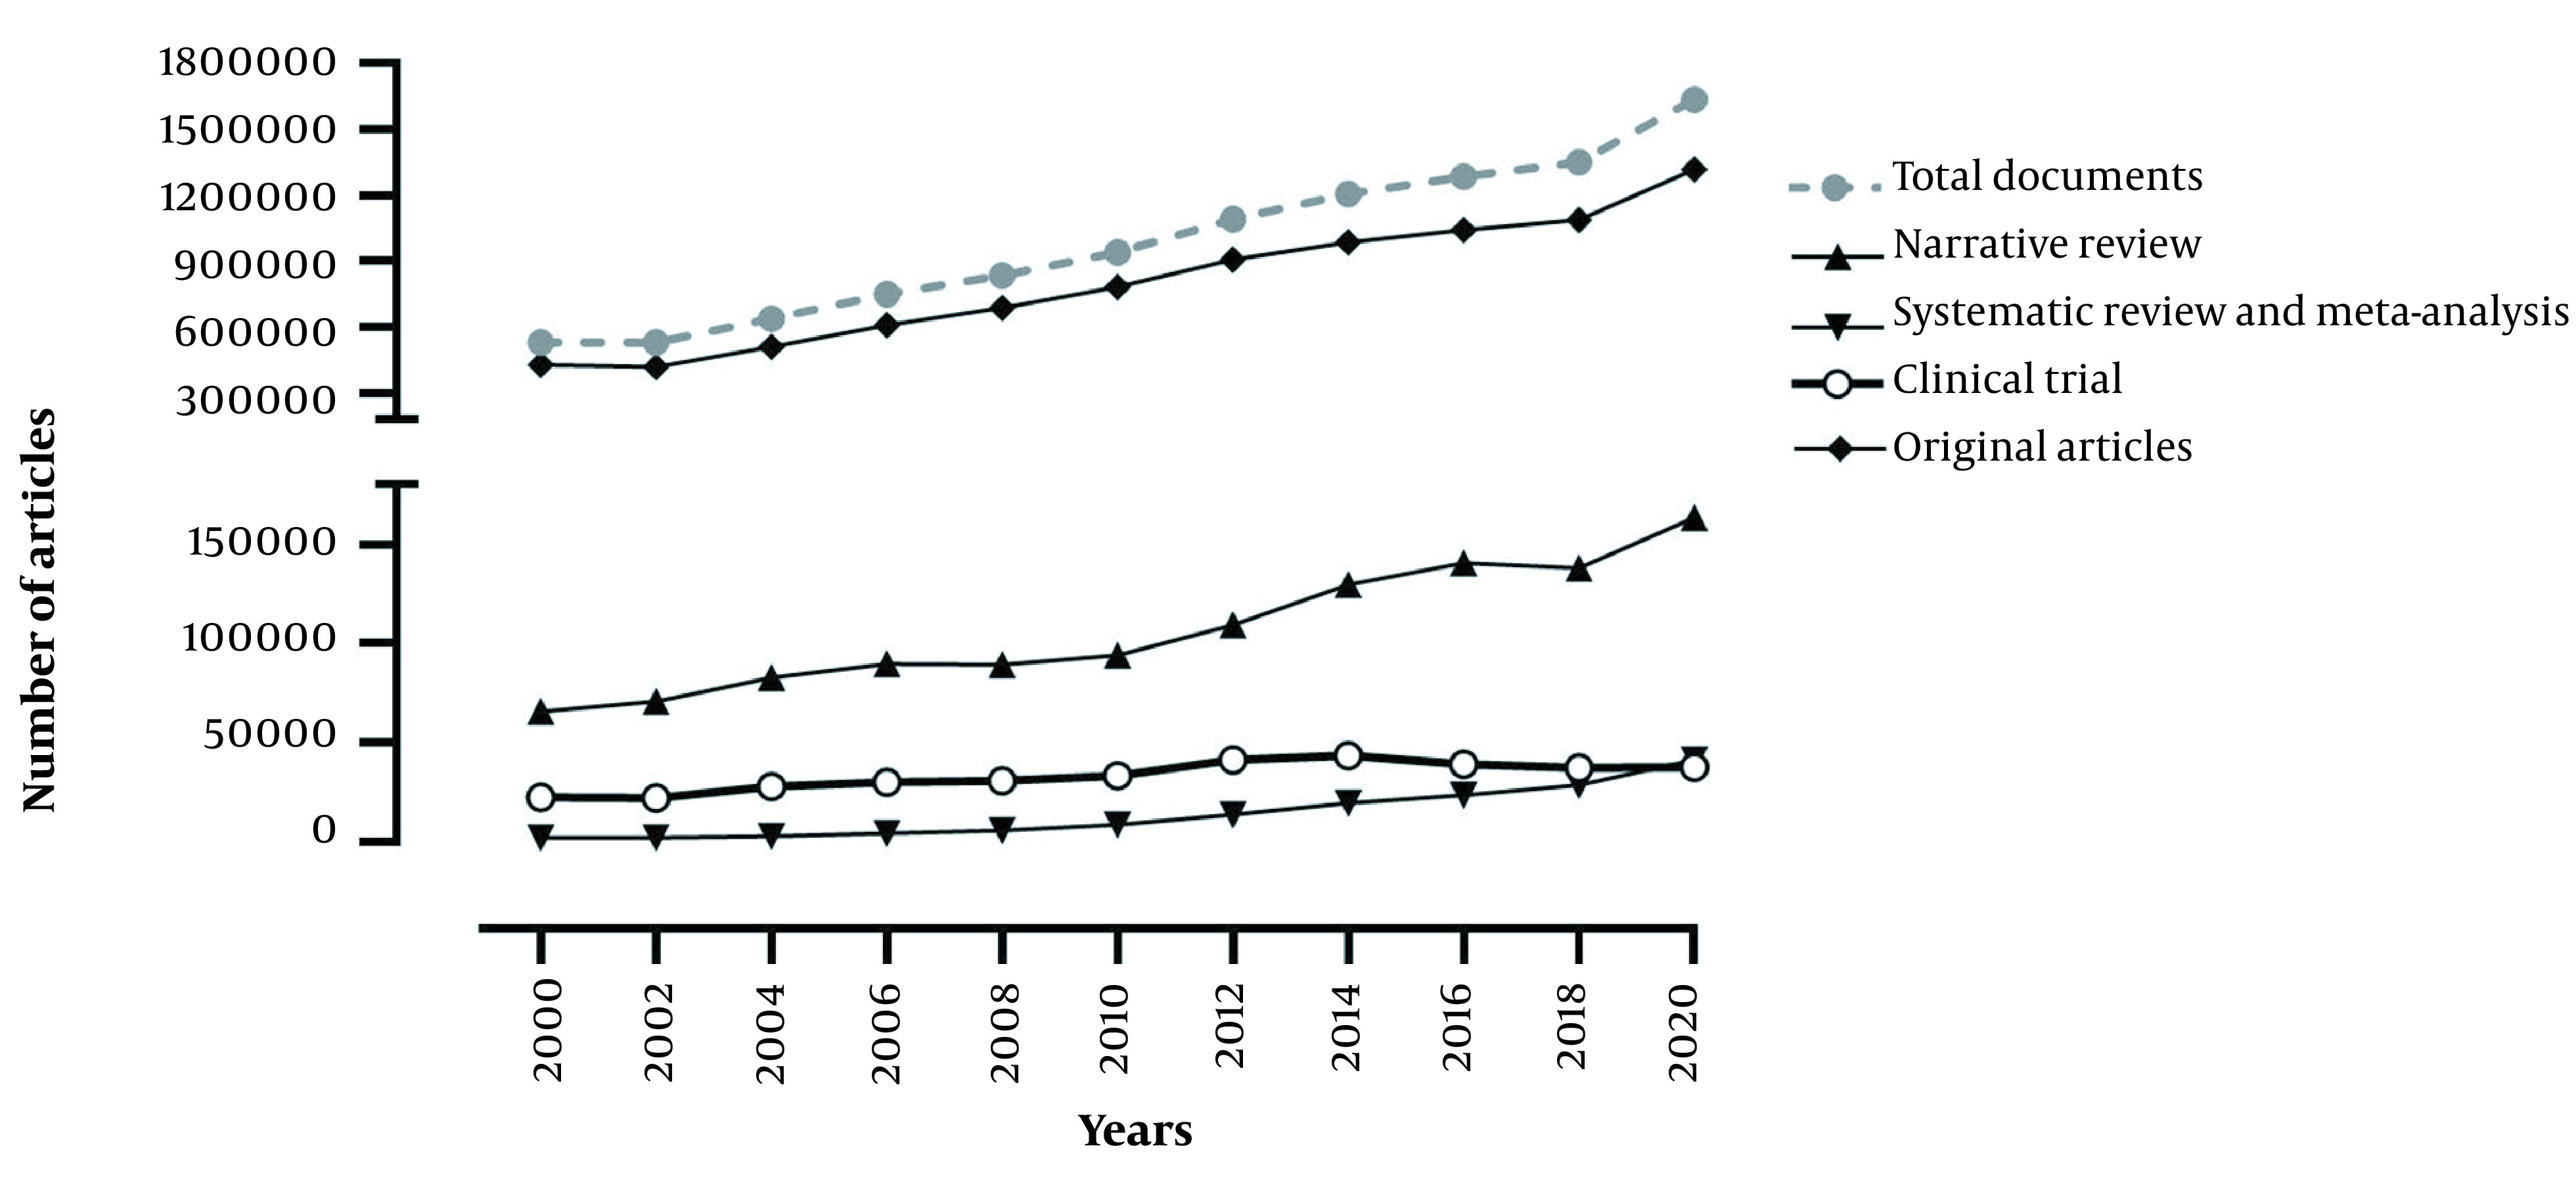
\includegraphics[width=1\linewidth]{images/increase_in_publications.jpg}
    \caption{Increasing publications over that past two decades \cite{ghasemi_scientific_2022}}
    \label{fig:increasing_publications_over_time}
\end{figure}

The publication rate of systematic reviews in medicine has surged exponentially in recent decades, reflecting their growing centrality to evidence-based practice. Between 1986 and 2015, PubMed documented a 2728\% increase in articles labeled as systematic reviews—far outpacing the 153\% rise in other publications during the same period  \cite{ioannidis_mass_2016}. This expansion reflects a pressing demand for consolidated, high-quality evidence to address diverse clinical questions, particularly as the volume of primary research grows. For instance, the number of clinical trials—a key source of evidence—doubled between 2001 and 2020, paralleled by a near-tripling of peer-reviewed journals \cite{ghasemi_scientific_2022}; see Figure \ref{fig:increasing_publications_over_time}). Methodological advances, such as PRISMA guidelines and GRADE frameworks, have further strengthened their rigor, enabling systematic reviews to shape clinical guidelines, inform policy, and even synthesise overlapping evidence through umbrella reviews. Organizations like Cochrane exemplify this impact: its 9,000+ systematic reviews, accessed over 17.5 million times by 2023, highlight their global reach and influence, underscored by a journal impact factor of 8.8\footnote{https://www.cochrane.org/about-us/scientific-strategy}.


\subsubsection{Process}

% Brief overview of the Cochrane Review process, and the characteristics of the process.
As elluded to, the process of producing a medical systematic review does not have a universally true process, as there are multiple forms of systematic review (i.e., Joanna Brigs Institute review (JBI), Network Meta-Analysis (Hoaglin et al 2011) or meta analysis (Gurvitch et al.)) \cite{munn_what_2018}. However, a commonly used systematic review process is the Cochrane Review \cite{cipriani_what_2011}. A Cochrane systematic review is characterised by:
\begin{itemize}
    \item {\bf{Standardised methology:}} SRs are often framed using a PICO format (Patient, Intervention, Comparison, Outcome). All reviews follow strict guidelines which are outlined in the Cochrane Handbook, ensuring a consistent approach to the review process. The process aims to minimise bia through methods like dual study selection, and data extraction by mutliple authors.
    \item {\bf{Mandatory Protocol Registration:}} Cochrane reviews necessitate the registration of the protocol before the review commences, reducing bias from post-hoc changes \cite{cumpston2024planning}.
    \item {\bf{Regular Updates:}} Cochrane systematic reviews are updated periodically, ensuring new evidence relevance. 
    \item {\bf{GRADE framework for evidence certainty:}} A system that rates certainty of evidence (high, moderate, low, very low) in summary of findings table \cite{schunemann2024summary}.
\end{itemize}

Specificially regarding this PhD, another beneficial characteristic of Cochrane reviews is that all processes are outlined in detail, making automation of these processes possible. 


% Focus on the search process within Cochrane reviews.

Information retrieval is utilised at numerous stages within producing a Cochrane review. Typically, the process is broken down into five distinct phases, as outlined in  Table \ref{tab:stages_of_sr}.
My PhD will focus on stage 2: Identifying relevant work, which can be further granularised into several substages:

\begin{itemize}
    \item Inclusion/exclusion criteria generation
    \item Search strategy development
    \item Database searching
    \item Protocol writing
    \item Title and abstract screening
    \item Full-text download and screening
    \item Manual search
\end{itemize}

Figure \ref{fig:selection_and_screening} illustrates these substages.

% Focus on the title and abstract screening substage.
Specifically, this PhD will concentrate solely on the title and abstract screening substage of the "identifying relevant work" phase. At this point in the identification of works process, preliminary work has been identified through a Boolean search, providing a large list of potentially included research. Traditionally, the titles and abstracts of these works are then manually evaluated by 2-3 reviewers to decide whether they should be included or excluded based on predetermined criteria, reducing the additional work that occurs within the full text download and screening substage. This process is similar to information retrieval.


\begin{table*}[t]
\centering
\small
\begin{tabular}{|c|p{0.85\textwidth}|}
\hline
\textbf{Stage} & \textbf{Purpose} \\
\hline
1 & \textbf{Framing questions for a review:} The research question is structured and explicitly formulated. \\\hline
2 & \textbf{Identifying relevant work:} A wide range of databases are searched to identify research to be included. Potential research is first identified, screened, eligibility checked, and then a decision is made on the inclusion of that research \cite{tawfik_step_2019}. \\\hline
3 & \textbf{Assessing the quality of studies:} Research is tested for quality, such as minimum research design, and subjected to higher quality assessment checks, including tests for research heterogeneity. \\\hline
4 & \textbf{Summarizing the evidence:} Data synthesis occurs with tabulation of study characteristics and quality. Statistical testing is performed at this stage. \\\hline
5 & \textbf{Interpreting the findings:} Any issues highlighted in the previous steps should be addressed. Generate recommendations guided by reference to the strength of the evidence. \\
\hline
\end{tabular}
\caption{Stages of a Systematic Review}
\label{tab:stages_of_sr}
\end{table*}

\subsubsection{Challanges}

% The need to improve efficiency in SRs is based on two main areas: the increasing volume of research and the resources available within healthcare care. It is known that the amount of research available to be included in these SRs is increasing; with an estimated number of peer-reviewed journals in 2020 being 46,739 (from 14, 694 in 2001), and the total number of articles published increasing threefold, and the total number of clinical research trials increasing twofold - 


see Figure \ref{fig:increasing_publications_over_time} \cite{ghasemi_scientific_2022}. However, the merits and disadvantages of the SR process are outside the scope of this Ph.D., but it has been succinctly conveyed in the existing literature \cite{howick_front_2011}, and, notwithstanding, SRs represent the best approach available to providing EBM.




Abstract screening averages 0.13-2.88 abstracts per minute \cite{shemilt_use_2016, giummarra_evaluation_2020, felizardo_visual_2013}. Conflict resolution, which is often necessary when multiple reviewers are used (which is preferred), takes on average 5 minutes. Screening a full-text article takes 4 minutes on average \cite{shemilt_use_2016}. Given a recently released Cochrane SR on the use of preoperative statin therapy in adults undergoing cardiac surgery, we can estimate that the total time to review all the text and abstracts for this would take 7.43 hours at best and 164.64 hours at worst \cite{antunes_preoperative_nodate}. Factored into an inflation adjusted average research cost per minute (£1.598), expected costs \textbf{for just this substage alone} could be expected to be £721.97 to £15,785.68 \cite{nussbaumer-streit_resource_2021}.

\subsubsection{Existing Automated Systems}

\subsection{Continuous Active Learning}
Active Learning (AL) presents a promising approach to address one of the most resource-intensive stages of the SR: title and abstract screening. In the context of SRs, where the volume of potentially relevant literature is vast and growing, AL offers a method to significantly reduce the manual workload while maintaining high accuracy in document selection.
Traditional systematic review methods require domain experts to manually screen all titles and abstracts identified in the initial search phase. This process is time-consuming and costly, especially given the increasing volume of published research. AL aims to optimise this process by intelligently selecting which documents should be reviewed by human experts, potentially saving significant time and resources.
By applying AL techniques to the screening process, we can:
\begin{itemize}
    \item Prioritise potentially relevant documents for expert review
    \item Reduce the overall number of documents that require manual screening
    \item Potentially identify relevant documents that might be missed in manual screening due to human fatigue or error
    \item Accelerate the overall SR process without compromising on quality
\end{itemize}

Deep-learning models have traditionally relied on large-labelled datasets for training. However, this approach contrasts sharply with real-world scenarios, particularly in specialised domains such as medicine. Although data collection is relatively straightforward in these fields, labelling is often time-consuming and requires expert knowledge \cite{smith_less_2018, hoi_batch_2006}. This disparity presents a significant challenge to optimise model performance with a limited number of labelled examples. This challenge is particularly relevant to the screening process in SRs, where we currently ask experts to screen all titles and abstracts returned from the identification phase. However, we would want to move to a scenario where minimal expert screening is sought from research returned from the identification phase, whose screening can then be safely extrapolated to a larger pool.

Active learning (AL) studies how to do just this. Through AL terms, it attempts to use a sampling policy $\pi$ to select samples $\mathbf{T}{C,i}$ from an unlabelled dataset $\mathbf{T}{U,i}$ and pass them to an oracle for labelling and added to a known dataset $\mathbf{T}_{K,i}$. Technology-Assisted Review (TAR), also known as Computer-Assisted Review or Predictive Coding, is a process that uses machine learning to assist in document review tasks. In the context of SRs, the TAR applies AL principles to streamline the selection process of titles and abstracts to screen. By iteratively training a machine learning model on human-labelled examples, TAR can prioritise potentially relevant documents for expert review, significantly reducing manual workload and, in some cases, exceeding human ability \cite{grossman_technology-assisted_2010}. This approach aligns closely with the goals of AL in SRs, as it aims to maximise the efficiency of expert input while maintaining high accuracy in document classification. 

Different approaches can be taken to AL, such as membership query synthesis \cite{angluin_queries_1988}, stream-based selective \cite{akinseloyin_novel_2024} and pool-based sampling \cite{lewis_sequential_1994}. These approaches are divided on how much of the unlabelled dataset ($\mathbf{T}{U, i}$) that a model has access to when utilising a policy $\pi$ for the selection of data points to be labelled $\mathbf{T}{C,i}$. In pool-based sampling, the entire unlabelled dataset, $\mathbf{T}{U,i}$, is evaluated in the selection of $\mathbf{T}{C,i}$, in stream-based selective sampling, datapoints are evaluated one at a time, and in membership query synthesis, synthetic data are generated from an underlying natural distribution. As we are concerned solely with the subprocess of title and abstract screening, it aligns strongly with pool-based sampling as the entire unlabelled dataset is known ahead of time and will be the approach used within this PhD. Figure \ref{fig:pool_based_query} outlines the AL cycle with pool-based querying.

\begin{figure}
\centering
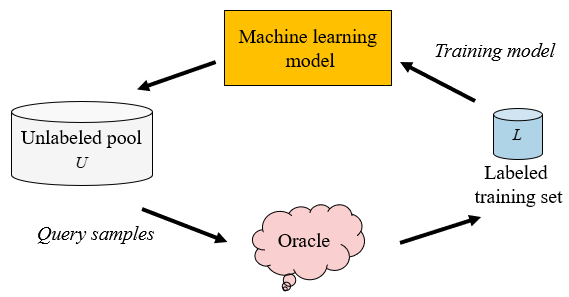
\includegraphics[width=0.5\linewidth]{images/pool_based_strategy.png}
\caption{Overview of a pool-based query strategy for AL, replicated\cite{ren_survey_2021}}.
\label{fig:pool_based_query}
\end{figure}

The oracle ($O$) within this PhD will denote a human-verified label resulting from screening potential research for inclusion within the SR within the title and abstract screening stage. Domain experts typically perform this. More concretely, $O$ can be considered a function $O(x) = y$ where $X$ is a representation, such as embedding the research title and abstract, and $y$ is the assigned category (included or excluded). We assumed that for each datapoint ($x$), $O$ provides a single judgement ($y$), which is always correct and do not concern ourselves with any potential intercoder agreement or bias within that decision process \cite{artstein_survey_2008}.

The broader literature has evaluated the effects of the choice of $\pi$. Traditionally, $\pi$ used the sigmoid response of the final layer of a model as a proxy of confidence, which is not a reliable measure, as these responses tend to be overly confident \cite{pearce_understanding_2021}. The use of the softmax response has been shown, in some cases, to be worse than random sampling \cite{wang_new_2014}. However, the effect of the choice of $\pi$ in combination with the final output layer in this specific domain (i.e. the SR process) is unknown, and this remains an active area of research which will not be covered during the PhD. The author uses techniques such as temperature scaling to effectively combat overly confident soft-max responses \cite{guo_calibration_2017}.


\begin{table*}[t]
    \centering
    \footnotesize

    \begin{tabular}{|c|c|>{\raggedright\arraybackslash}p{11cm}|}
        \hline
        \textbf{Notation}    & \textbf{Explanation}                            & \textbf{Notes}                                                                                \\
        \hline
        \(\textbf{T}\)       & Total dataset                                   & e.g. Research gathered after Identification phase of the selection process.                   \\
        \hline
        \(i\)                & Iteration                                       & A single cycle within the active learning process.                                            \\
        \hline
        \(\textbf{T}_{K,i}\) & Known datapoints per iteration                  & e.g. research that has been screened by a reviewer                                            \\
        \hline
        \(\textbf{T}_{U,i}\) & Unknown datapoints per iteration                & e.g. research that has not been screened by a reviewer                                        \\
        \hline
        \(\textbf{T}_{C,i}\) & A subset of \(\textbf{T}_{U,i}\) to be labelled & chosen by a policy, datapoints to be screened by a reviewer.                                  \\
        \hline
        $\pi$                & Policy                                          & How \(\textbf{T}_{U,i}\) is selected, e.g. uncertainty, random, certainty, diversity sampling \\
        \hline
        O                    & Oracle                                          & Often a domain expert, who assigns labels to unscreened research.                             \\
        \hline
        \(T_R\)              & Total Relevant Documents                        & All research that should be included in a systematic review.                                  \\
        \hline
        \(T_{IR}\)           & Total Irrelevant Documents                      & All research that should not be included in a systematic review.                              \\
        \hline
    \end{tabular}
    \caption{Notation used for active learning within this review}
    \label{tab:notation}
\end{table*}


In the author's mind, it is unclear the exact difference between continuous/online active learning (CAL) and AL, and indeed, it seems that much of the current literature refers to CAL when, in fact, it means AL. Some authors refer to eliminating models between iterations and the process occurring in discrete rounds as AL \cite{settles_active_2009}. Cormack differentiates the two based on objectives, with the aim of CAL being to find and review as many of the responsive documents as possible, as quickly as possible, and AL is to produce the best classier possible, considering the level of training effort (which are subtlely different objectives) \cite{cormack_autonomy_2015}. For this research, we will use continuous to denote the incremental streaming of newly available information to any model. 

There exists a plethora of research within the AL area; however, due to the specific focus on medicine within this PhD, I will focus on existing literature within the medical domain and some key ones from others. It is valid to delineate between research within differing domains within AL (e.g., e-discovery in the Legal Domain, sentiment analysis on social media, or image classification in computer vision) as each domain presents unique challenges and characteristics that influence the application of AL techniques. In the medical domain, particularly in SRs, AL must contend with highly specialised vocabulary, complex interrelationships between concepts, and the critical importance of high recall to ensure that relevant studies are not missed.
The emphasis of the medical domain on evidence-based practice and the potential impact on patient care requires a more stringent approach to AL. Unlike other domains, where missing a small percentage of relevant items might be acceptable in systematic medicine reviews, overlooking a crucial study could have significant consequences. This requirement for near-perfect recall and the need to process large volumes of literature efficiently create a unique set of demands for medical TAR AL algorithms. This literature review will assess each work for their respective contributions, the datasets used, the evaluation metrics (and scores achieved), the models used, and the representation of data points used in each approach.

An early contribution to this field demonstrated that automated classification of document citations can be used to reduce the time reviewers spend screening evidence for inclusion in SRS of drug class efficacy \cite{cohen_reducing_2006}. The researchers used a novel data set created from annotated reference files from 15 SRs of drug classes. The features were extracted from the research articles using the "bag-of-words" approach for the title and abstract, the MeSH terms, and the MEDLINE publication type. The features were one-hot encoded and selected using the chi-square test to drop insignificant features. Finally, this input was used to train a perceptron model and was evaluated using precision, recall, and the F measure in a range of sample weighting and the WSS@95\%. This work's significant contribution was using machine learning approaches to address this screening issue.

A significant contribution to the field came from a simulation study that mimics the process of a human reviewer screening records while interacting with an active learning model \cite{ferdinands_performance_2023}. This work used six previously labelled SRs. It looked at four classification techniques (naive Bayes, logistic regression, support vector machines, and random forest). Two feature extraction strategies (TF-IDF and doc2vec) were evaluated based on the work saved on sampling and recall. The title and abstracts were used to generate these inputs. It showed that in a simulated approach, the models reduced the number of publications screened from 91.7 to 63. 9\% (WSS@95). The naive Bayes and TF-IDF models yielded the best overall results in this study. This study is limited due to the smaller datasets used and the feature extraction approaches used (which, for the year of publication, other potential superior choices, such as contextual embeddings, could have been explored). It introduced some new evaluation metrics, such as TTD and ATD. This research only superficially evaluates the variability of these approaches in SRs, reporting the range of WSS@95 and not attempting to consider factors within SRs that may have led to this variability. 

More recent work reported a protocol denoted ``CAL'' (Continuous Active Learning), initially performed on legal datasets \cite{cormack_evaluationsections//_2014}. The process involves selecting an initial set of seed documents, typically using keyword search, which are then reviewed and coded. This training set is used to train a model that scores each document based on its response (relevant) likelihood. The top-scoring documents that have not been coded are then reviewed and coded. The extended training set is then used to retrain the model, and this process continues until ``enough'' of the responsive documents are found.
The key difference between this approach and previous ones, such as SAL (Simple Active Learning) and SPL (Simple Passive Learning), is their selection strategy: CAL uses relevance feedback (selecting highest-scoring documents), SAL uses uncertainty sampling, and SPL uses random selection. CAL achieved better results on the recall@75 \% metric, which measures the effort required to achieve 75\% recall.
The study primarily used SVM (Sofia-ML implementation of Pegasos SVM) for all protocols. It mentions briefly that it replicated most experiments using logistic regression, achieving similar results to SVM. It also tested with Nave Bayes, which achieved generally inferior results overall but maintained the same relative effectiveness among the protocols.
This paper is essential to outline the CAL process and demonstrate its effectiveness. However, it had some limitations: It used a fixed batch size of 1,000 documents for efficiency, though they noted slightly better results with a batch size of 100 for CAL. Although multiple classifiers were tested, detailed performance comparisons between models were not reported. The study did not explore extensively the effects of feature engineering methods. The human factors in review accuracy were not fully addressed in the simulation. Despite these limitations, the article provided a strong foundation for understanding and further investigating TAR protocols in SR TAR.

The follow-up was to introduce the autonomous TAR process (Auto TAR), which showed better performance than CAL \cite{cormack_autonomy_2015}. The algorithm is outlined in Figure \ref{fig:autotar_process}. 
The AUTO TAR process differs from CAL through:
\begin{itemize}
    \item AUTO TAR uses a single seed document, and CAL uses a 1,000 document set.
    \item AUTO TAR uses word-based features TF-IDF, and CAL uses binary byte-4 grammes.
    \item AUTO TAR exponentially increases batch sizes, starting with one and increasing by 10\% each iteration; CAL's batch size is fixed at 1,000
\end{itemize}

\begin{figure}
    \centering
    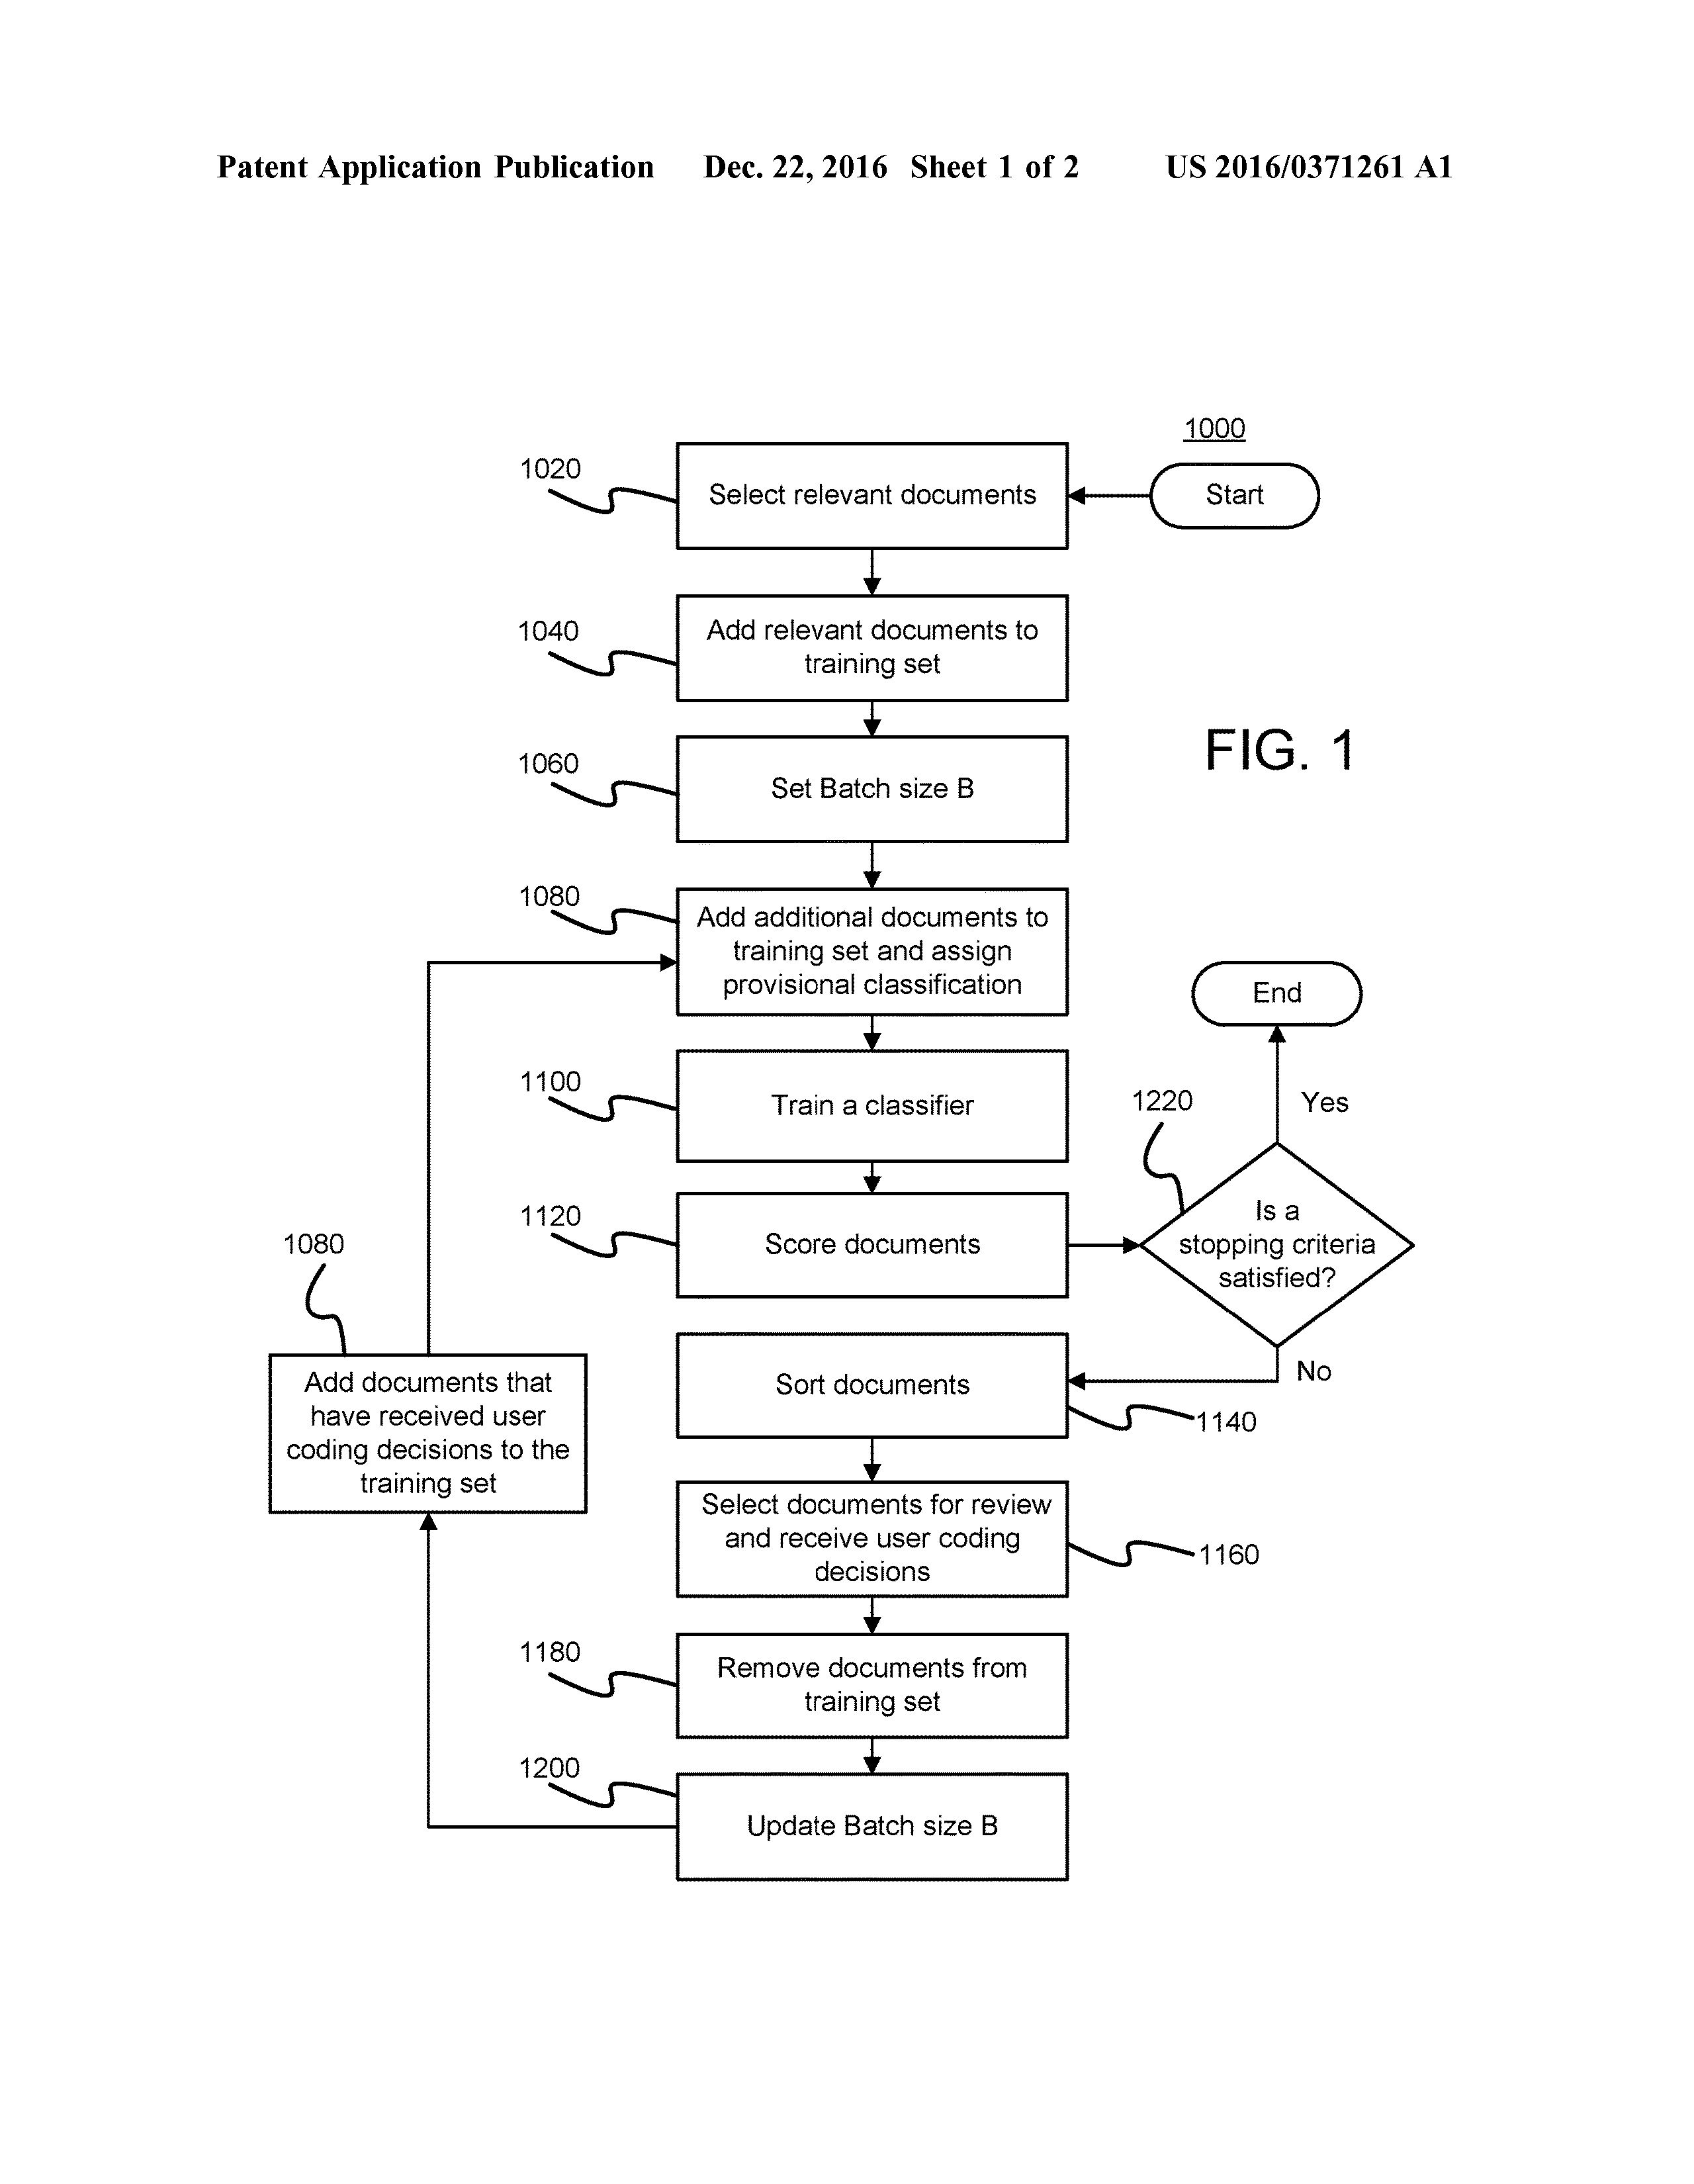
\includegraphics[width=1\linewidth]{images/autotar.jpg}
    \caption{Auto TAR outline, as documented within the patient filing by Cormack et al. \cite{cormack_systems_2016}}.
    \label{fig:autotar_process}
\end{figure}
Finally, this approach was augmented to use BM25 (a saturated form of TF-IDF) + logistic regression and has been considered state-of-the-art for the past eight years. This is often referred to as "base model implementation", or abbreviated to BMI.

Since 2016's AutoTar approach, the transformer architecture has advanced virtually all fields within natural language processing, permeating almost every aspect of the field \cite{vaswani_attention_2023}. However, the TAR process has remained surprisingly resistant to these advances. Although a comprehensive analysis of transformer-based improvements is beyond the scope of this literature review, their primary advantage is their ability to provide a nuanced contextual understanding of written texts.
This contextual comprehension differs significantly from traditional feature extraction techniques such as TF-IDF. Transformers employ self-attention mechanisms to learn context-dependent text representations, enabling them to capture subtle semantic relationships and long-range dependencies not present with TF-IDF-like approaches, in the TAR process.

\hl{Add in about CALBERT}


Subsequent research using decoder architectures within CAL attempted to understand why their performance was underwhelming compared to BMI. 
Goldilocks \cite{yang_goldilocks_2022} took a pre-trained BERT model and fine-tuned it first on the unlabelled corpus (0-10 epochs were tested). They then randomly selected a positive example seed, and on each iteration of the AL process 200 documents were sampled using either relevance feedback or uncertainty sampling. During each iteration, after labelling, all labelled documents were used to fine-tune BERT again for 20 epochs, using the previous model from the previous iteration as the starting point. The input was the concatenated title and body text, truncated to 512 tokens. The model was then used to classify a document's relevance. They found that 5-epoch fine-tuning on the unlabelled dataset was "just right", and achieved similar performance to that of TF-IDF \& logistic regression within domain dataset (RCV1-V2 corpus), and statistically significantly worse on out-of-domain dataset(Jeb Bush corpus). Although not discussed in the paper, this could be explained through the phenomenon of "catastrophic forgetting", where too much fine-tuning on the task corpus might cause the model to forget useful general knowledge from pertaining \cite{xu_forget_2020}. Additionally, they used the model from the previous iteration as a starting point for new classification fine-tuning iterations, which could have further compounded this. 

However, the concept of a "goldilocks" epoch for CAL within medical data sets did not seem to hold, with subsequent research demonstrating that a "just right retaining epoch" was not present in the CLEF data set \cite{noauthor_ielabgoldilocks-reproduce_2024}. 

\hl{Issues with Goldilocks:}
\begin{enumerate}
    \item Contrived experimental design.
    \item Sensitive to pre-trained model choice.
\end{enumerate}

\subsection{Stopping Algorithms}

\section{RESEARCH QUESTIONS}


\subsection{Leveraging Citation Networks for Medical TAR}

Systematic reviews utilise research evidence to provide clinical practice recommendations. The communication of medical research follows standardised formatting conventions and primarily occurs through peer-reviewed publication \cite{BMCMedicalResearch}. When authors compose research papers, they must reference related works to substantiate their claims and situate their findings within the existing body of knowledge. These citations follow standardised formatting guidelines and are documented in the paper's reference section. This rigorous documentation of citations enables analysis of the relationships between research papers, operating under the assumption that studies that cite or are cited by a research article are relevant to that research.

\subsubsection{Relation analysis improves CAL TAR performance}

Recent advances in medical CAL TAR have indirectly demonstrated the benefit of relationship analysis for citations. The current leading encoder model, $BioLinkBERT_{base}$ achieved state-of-the-art performance on the CLEF dataset in a CAL setting by leveraging citations networks between research papers \cite{yasunaga2022linkbertpretraininglanguagemodels, goharian_reproducibility_2024}. 


The $LinkBERT$ approach was to view a pertaining corpus as a graph of documents, with each document being a vertex and hyperlinks forming edges between documents. These related documents were then placed within the same context window. The approach differs from traditional $BERT$ architectures, which randomly allocate documents to context windows without considering their relationships. While this might appear similar to curriculum learning approachings, $LinkBERT$ is distinct in that it does not organise context windows by difficulty level. 

$BioLinkBERT$, a domain-specific adaption of $LinkBERT$, was developed specifically for biomedical aplications and pretrained exclusively on PubMed articles, using citation relationships to estimate document relationships \footnote{https://huggingface.co/michiyasunaga/BioLinkBERT-base}. The model trianing process incorporated standard masked language modelling and next-sentence prediction techniques. Analysis of both the base model (100M parameters) and large model (340M parameters) against $PubMedBERT$ across multiple benchmarks:  BLURB\cite{guDomainSpecificLanguageModel2021}, MedQA-USMLE\cite{jinWhatDiseaseDoes2020}, and MMLU-professional medicine\cite{hendrycksMeasuringMassiveMultitask2021}. The results demonstrated $BioLinkBERT_{large}$'s superior performance across all evaluated benchmarks, notably achieving a 3.2\% improvement over PubMedBERT in the BLURB score.


\begin{figure}[t]
    \centering
    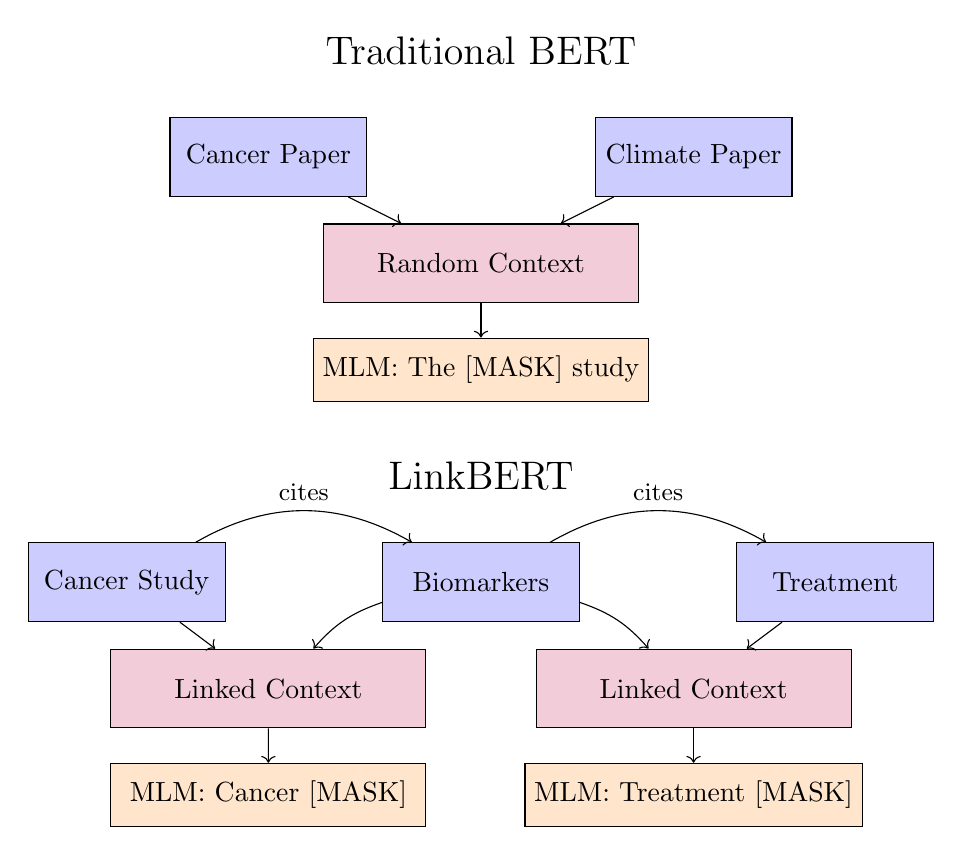
\begin{tikzpicture}[
        doc/.style={rectangle, draw, fill=blue!20, minimum width=2.5cm, minimum height=1cm},
        window/.style={rectangle, draw, fill=purple!20, minimum width=4cm, minimum height=1cm},
        mlm/.style={rectangle, draw, fill=orange!20, minimum width=4cm, minimum height=0.8cm},
        node distance=2cm,
        scale=0.9
    ]
    % Traditional BERT (top)
    \node[align=center] at (-3,5) {\Large Traditional BERT};
    \node[doc] (a1) at (-6,3.5) {Cancer Paper};
    \node[doc] (a2) at (0,3.5) {Climate Paper};
    \node[window] (b1) at (-3,2) {Random Context};
    \node[mlm] (m1) at (-3,0.5) {MLM: The [MASK] study};
    
    \draw[->] (a1) -- (b1);
    \draw[->] (a2) -- (b1);
    \draw[->] (b1) -- (m1);
    
    % LinkBERT (bottom) - with increased horizontal spacing
    \node[align=center] at (-3,-1) {\Large LinkBERT};
    \node[doc] (c1) at (-8,-2.5) {Cancer Study};
    \node[doc] (c2) at (-3,-2.5) {Biomarkers};
    \node[doc] (c3) at (2,-2.5) {Treatment};
    
    \node[window] (d1) at (-6,-4) {Linked Context};
    \node[mlm] (n1) at (-6,-5.5) {MLM: Cancer [MASK]};
    
    \node[window] (d2) at (0,-4) {Linked Context};
    \node[mlm] (n2) at (0,-5.5) {MLM: Treatment [MASK]};
    
    % Citations with curved arrows
    \draw[->, bend angle=30] (c1) to[bend left] node[midway,above] {\small cites} (c2);
    \draw[->, bend angle=30] (c2) to[bend left] node[midway,above] {\small cites} (c3);
    
    % Context connections with slight bends to avoid overlap
    \draw[->] (c1) -- (d1);
    \draw[->] (c2) to[bend right=15] (d1);
    \draw[->] (c2) to[bend left=15] (d2);
    \draw[->] (c3) -- (d2);
    \draw[->] (d1) -- (n1);
    \draw[->] (d2) -- (n2);
    
    \end{tikzpicture}
    \caption{Comparison of document processing in traditional BERT versus LinkBERT. Traditional BERT (top) randomly groups documents into context windows, while LinkBERT (bottom) uses citation relationships to create meaningful document groupings for pretraining. The citation-based grouping ensures that semantically related documents are processed together during masked language modeling tasks.}
    \label{fig:linkbert-comparison}
\end{figure}


Current research on document relationship-based encoders in the CAL process has not definitively established that document relations are the primary driver of performance improvements. Furthermore, the assumption that larger models consistently yield better results is not always the case. The author replicated the previously reported Goldilock Reproduce study, where $BioLinkBERT_{base}$ formed the classifier, except changing the model to the $BioBERT_{large}$ variant\footnote{https://huggingface.co/michiyasunaga/BioLinkBERT-large} as a classifier model, yet only achieved higher performance in R-Precision in 7 of 12 datasets/policy combinations.  The empirical results, detailed in Table \ref{tab:results-average}, show peak R-precision values of 0.847 for the relevancy selection policy (at FPT epoch 2) and 0.832 for uncertainty selection (at FPT epoch 1).Statistical analysis using the Friedman test revealed significant differences between Further Pre-Training (FPT) epochs in only 4 of 12 datasets when examined individually. More importantly, when analyzing all datasets collectively, no statistically significant differences emerged in R-precision values across FPT epochs for either relevancy selection or uncertainty selection policies. This findiing challenges the previously documented  ``Goldilocks problem'' observed in non-medical domains. Specifically demonstrating that FPT does not yield statistically significant improvemnts in R-Precision. 

This replication study has generated valuable insights for this PhD investigation. A significant finding indicates that seeking an optimal pretraining epoch within the CLEF dataset is unlikely to be productive for future research endeavors. The experimental design revealed several methodological considerations, particularly regarding the implementation of hyperparameters without robust empirical justification. These include the selection of a batch size of 25, the decision to fine-tune for 20 epochs, and the termination criterion of 501 labeled documents. These parameter choices, while functional, may impose limitations on potential improvements to encoder CAL process performance within the experimental framework.

The significance of these limitations becomes particularly evident when considering that observed R-Precision values approach the theoretical maximum of 1.0, with some instances achieving values as high as 0.945. In the context of the Goldilocks reproduce paper, datasets showing lower performance metrics, such as the CLEF 2019 dataset (with R-precision values of 0.82 for relevancy and 0.791 for uncertainty), present additional analytical challenges. The utilization of Large Language Models (LLMs) introduces complexity in interpreting the underlying causes of reduced performance in these cases.

While exploring larger, more sophisticated models presents a potential avenue for improvement, this approach faces practical constraints. Given the limitations of High-Performance Computing resources and PhD time constraints, pursuing research dependent on the development and availability of superior LLMs may not be the most pragmatic direction.

A crucial observation emerged from this research regarding the relationship between early document classification and overall performance. In iterations where strong performance was ultimately achieved at iteration 20, a notably higher number of relevant documents were classified earlier in the CAL process. This finding aligns with theoretical expectations: a larger corpus of correctly classified documents early in the process provides a more robust foundation for subsequent classification decisions. This insight carries significant implications for the next phase of this PhD research, suggesting that enhancing document availability in the early stages of the active learning process could substantially improve overall performance outcomes.

While $BioLinkBERT$ represents a sophisticated approach that combines citation networks with contextual language understanding, this integration presents both advantages and limitations. The model's ability to capture complex semantic relationships between documents is valuable, but the contextual processing introduces potential inefficiencies. During pretraining, when linked documents are placed in the same context, the model must process all content within those documents—including sections that may be tangential or unrelated to the citing paper's specific reference. This contextual noise could potentially dilute the precision of the more direct relationships that citations inherently represent. In contrast, pure citation links directly capture intentional scholarly connections made by domain experts, providing a cleaner signal without the additional complexity of processing potentially irrelevant contextual information.

A fundamental question emerges from this research: Is contextual understanding of references truly necessary for effective CAL? Several factors suggest that citation networks alone might be sufficient and potentially superior. First, citations themselves represent a form of knowledge distillation, where domain experts have already identified meaningful relationships between documents. Second, analysing reference networks is computationally more efficient than processing full textual contexts. Third, citation network models tend to be more stable when updated, compared to contextual models. Fourth, the contextualization of citation networks may actually introduce noise into what would otherwise be clear citation signals.


\begin{table}[htbp]
    \centering
    \footnotesize
    \setlength{\tabcolsep}{4pt}
    \begin{tabular}{l>{\raggedright\arraybackslash}p{1.2cm}ccccc}
    \hline
    \textbf{Collection} & \textbf{Dataset size} & \textbf{Model} & \multicolumn{2}{c}{\textbf{R-Precision (↑)}} & \multicolumn{2}{c}{\textbf{Friedman (p)}} \\
    \cline{4-7}
    & & & \textbf{Rel.} & \textbf{Unc.} & \textbf{Rel.} & \textbf{Unc.} \\
    \hline
    \multirow{6}{*}{\makecell[l]{Clef 2019\\dta test}} & 
    \multirow{6}{*}{8} & BiolinkBert-Base-ep0 & \textbf{0.909} & \textbf{0.857} & \multicolumn{2}{c}{---} \\
    & & BiolinkBert-Large-ep0 & 0.897 & 0.803 & \multirow{5}{*}{0.914} & \multirow{5}{*}{0.632} \\
    & & BiolinkBert-Large-ep1 & 0.827 & 0.832 & & \\
    & & BiolinkBert-Large-ep2 & 0.812 & 0.774 & & \\
    & & BiolinkBert-Large-ep5 & 0.841 & 0.814 & & \\
    & & BiolinkBert-Large-ep10 & 0.881 & 0.846 & & \\
    \hline
    \multirow{6}{*}{\makecell[l]{Clef 2017\\test}} & 
    \multirow{6}{*}{30} & BiolinkBert-Base-ep0 & 0.812 & 0.794 & \multicolumn{2}{c}{---} \\
    & & BiolinkBert-Large-ep0 & 0.828 & 0.797 & \multirow{5}{*}{\textbf{\textless0.05}} & \multirow{5}{*}{\textbf{\textless0.05}} \\
    & & BiolinkBert-Large-ep1 & 0.826 & \textbf{0.827} & & \\
    & & BiolinkBert-Large-ep2 & \textbf{0.858} & 0.804 & & \\
    & & BiolinkBert-Large-ep5 & 0.827 & 0.777 & & \\
    & & BiolinkBert-Large-ep10 & 0.799 & 0.757 & & \\
    \hline
    \multirow{6}{*}{\makecell[l]{Clef 2017\\train}} & 
    \multirow{6}{*}{20} & BiolinkBert-Base-ep0 & \textbf{0.838} & 0.761 & \multicolumn{2}{c}{---} \\
    & & BiolinkBert-Large-ep0 & 0.778 & 0.765 & \multirow{5}{*}{\textbf{\textless0.05}} & \multirow{5}{*}{0.28} \\
    & & BiolinkBert-Large-ep1 & 0.808 & 0.789 & & \\
    & & BiolinkBert-Large-ep2 & 0.767 & 0.701 & & \\
    & & BiolinkBert-Large-ep5 & 0.816 & 0.786 & & \\
    & & BiolinkBert-Large-ep10 & 0.827 & \textbf{0.796} & & \\
    \hline
    \multirow{6}{*}{\makecell[l]{Clef 2018\\test}} & 
    \multirow{6}{*}{30} & BiolinkBert-Base-ep0 & 0.794 & 0.780 & \multicolumn{2}{c}{---} \\
    & & BiolinkBert-Large-ep0 & 0.789 & 0.774 & \multirow{5}{*}{0.52} & \multirow{5}{*}{0.50} \\
    & & BiolinkBert-Large-ep1 & \textbf{0.812} & 0.790 & & \\
    & & BiolinkBert-Large-ep2 & 0.797 & \textbf{0.791} & & \\
    & & BiolinkBert-Large-ep5 & 0.763 & 0.773 & & \\
    & & BiolinkBert-Large-ep10 & 0.763 & 0.769 & & \\
    \hline
    \multirow{6}{*}{\makecell[l]{Clef 2019\\DTA int.\\train}} & 
    \multirow{6}{*}{20} & BiolinkBert-Base-ep0 & 0.939 & 0.923 & \multicolumn{2}{c}{---} \\
    & & BiolinkBert-Large-ep0 & 0.939 & 0.902 & \multirow{5}{*}{0.78} & \multirow{5}{*}{0.50} \\
    & & BiolinkBert-Large-ep1 & 0.941 & 0.935 & & \\
    & & BiolinkBert-Large-ep2 & 0.948 & 0.921 & & \\
    & & BiolinkBert-Large-ep5 & 0.952 & 0.945 & & \\
    & & BiolinkBert-Large-ep10 & \textbf{0.945} & \textbf{0.947} & & \\
    \hline
    \multirow{6}{*}{\makecell[l]{Clef 2019\\DTA int.\\test}} & 
    \multirow{6}{*}{20} & BiolinkBert-Base-ep0 & \textbf{0.934} & \textbf{0.900} & \multicolumn{2}{c}{---} \\
    & & BiolinkBert-Large-ep0 & 0.899 & 0.856 & \multirow{5}{*}{0.87} & \multirow{5}{*}{\textbf{\textless0.05}} \\
    & & BiolinkBert-Large-ep1 & 0.904 & 0.840 & & \\
    & & BiolinkBert-Large-ep2 & 0.909 & 0.878 & & \\
    & & BiolinkBert-Large-ep5 & 0.882 & 0.835 & & \\
    & & BiolinkBert-Large-ep10 & 0.865 & 0.841 & & \\
    \hline
   
    \end{tabular}
    \caption{Performance comparison across different collections and models}
    \label{tab:results}
\end{table}

\begin{table}[htbp]
    \centering
    \caption{Average R-precision of each FPT epoch for CLEF dataset}
    \begin{tabular}{l>{\raggedright\arraybackslash}p{1.2cm}ccccc}
        \textbf{Policy} & \textbf{ep0} & \textbf{ep1} & \textbf{ep2} & \textbf{ep5} & \textbf{ep10} \\
        \hline
        Uncertainty & 0.813 & 0.832 & 0.813 & 0.815 & 0.814 \\
        Relevancy & 0.840 & 0.845 & 0.847 & 0.842 & 0.835 \\
    \hline

    \end{tabular}
    \label{tab:results-average}
\end{table}



\subsubsection{Direct citation network mining within medicine research}

Performant, simple, and robust approaches to citation network mining already exist within medicial research. Let G be a citation graph where:

\begin{itemize}
    \item $D_i$ represents a research article of interest as a vertex in G
    \item $D_{ip}$ represents the set of articles referenced by $D_i$
    \item $D_{if}$ represents the set of articles that reference $D_i$
    \item Both sets are subsets of G: $D_{ip}, D_{if} \subset G$
    \item $D_{ip} \cap D_{if} = \emptyset$, so searching both sets will provide different relevant articles
\end{itemize}

Relevancy is defined as a function $R: D \rightarrow [0,1]$, where:

\begin{itemize}
    \item 0 denotes no relevance
    \item 1 denotes maximum relevance
    \item For any set of documents $D_{set}$, relevancy is defined as $R(D_{set}) = {R(d) | d \in D_{set}}$
\end{itemize}

Two primary citation network mining approaches are defined:
\begin{itemize}
    \item Backward citation searching (BCS): examining all articles in $D_{ip}$\cite{lefebvre2011cochrane, akers2009systematic}
    \item Forward citation searching (FCS): examining all articles in $D_{if}$*\footnote{FCS involves using a citation index to identify studies that cite a source study. A citation index is a database of scholarly articles and their citations, such as PubMed, Google Scholar, Scopus or OpenAlex}
\end{itemize}

Backward and forward citation searching (BCS and FCS) are both straightforward and effective approaches that inherently respect the chronological relationships between research articles, as papers can only cite previously published work. The significance of these methods is demonstrated by their recommended use in Cochrane systematic reviews, particularly during the identification phase. A study of Cochrane reviews conducted between November 2016 and January 2017 found that 87\% reported using BCS, while 9\% utilized FCS \cite{briscoeConductReportingCitation2019}.. The Cochrane Handbook explicitly mandates the use of BCS (criterion C30) in the search stage, though it makes no mention of FCS  \cite{MECIRManualCochrane}. However, neither the use of BCS nor FCS is addressed in the Handbook's guidelines for the screening phase.


The application of Backward and Forward Citation Searching (BCS and FCS) within an active learning process represents an understudied area of research (see Figure \ref{fig:search-results} for search strategy details). To establish the novelty of this augmentation, several key distinctions must be clarified. While this PhD research focuses on the title and abstract screening phase of systematic review generation, BCS and FCS have traditionally been confined to the identification phase (as illustrated in Figure \ref{fig:selection_and_screening}). Conventionally, title and abstract screening serves to reduce the workload for the more resource-intensive full-text screening phase. However, from a computational perspective, restricting the screening process to titles and abstracts is unnecessary, as the computational cost remains manageable when including full texts.
 
\begin{figure}[htbp]
    \centering
    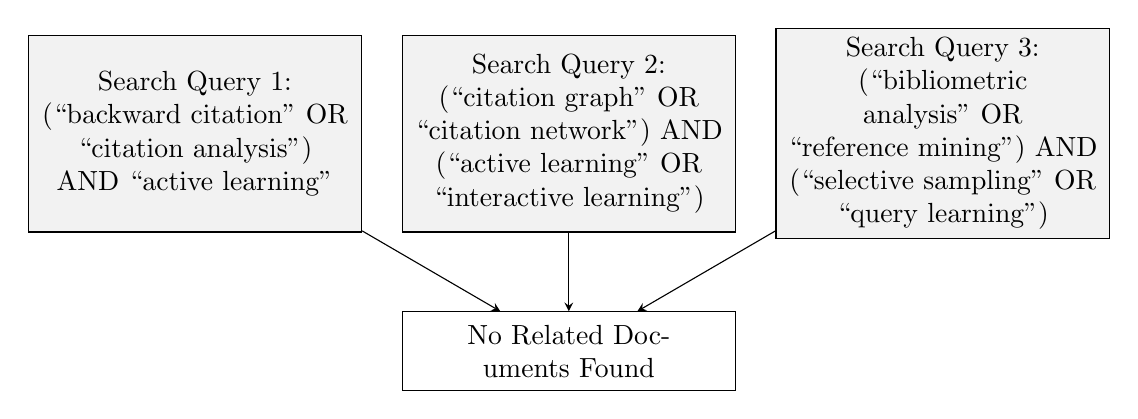
\begin{tikzpicture}[
        node distance = 0.5cm,
        box/.style={rectangle, draw, text width=4cm, minimum height=1cm, align=center},
        query/.style={rectangle, draw, fill=gray!10, text width=4cm, minimum height=2.5cm, align=center}
    ]
        % Search queries side by side
        \node[query] (q1) {Search Query 1:\\
            (``backward citation'' OR\\``citation analysis'')\\
            AND ``active learning''};
        \node[query] (q2) [right=0.5cm of q1] {Search Query 2:\\
            (``citation graph'' OR\\``citation network'') AND\\(``active learning'' OR\\``interactive learning'')};
        \node[query] (q3) [right=0.5cm of q2] {Search Query 3:\\
            (``bibliometric analysis'' OR\\``reference mining'') AND\\(``selective sampling'' OR\\``query learning'')};
            
        % Results box below
        \node[box] (results) [below=1cm of q2] {No Related Documents Found};
            
        % Arrows
        \draw[-stealth] (q1) -- (results);
        \draw[-stealth] (q2) -- (results);
        \draw[-stealth] (q3) -- (results);
        
    \end{tikzpicture}
    \caption{Results from literature search on citation index arxiv and pubmed demonstrating absence of related works, ran on 13th November 2024}
    \label{fig:search-results}
\end{figure}
\begin{center}
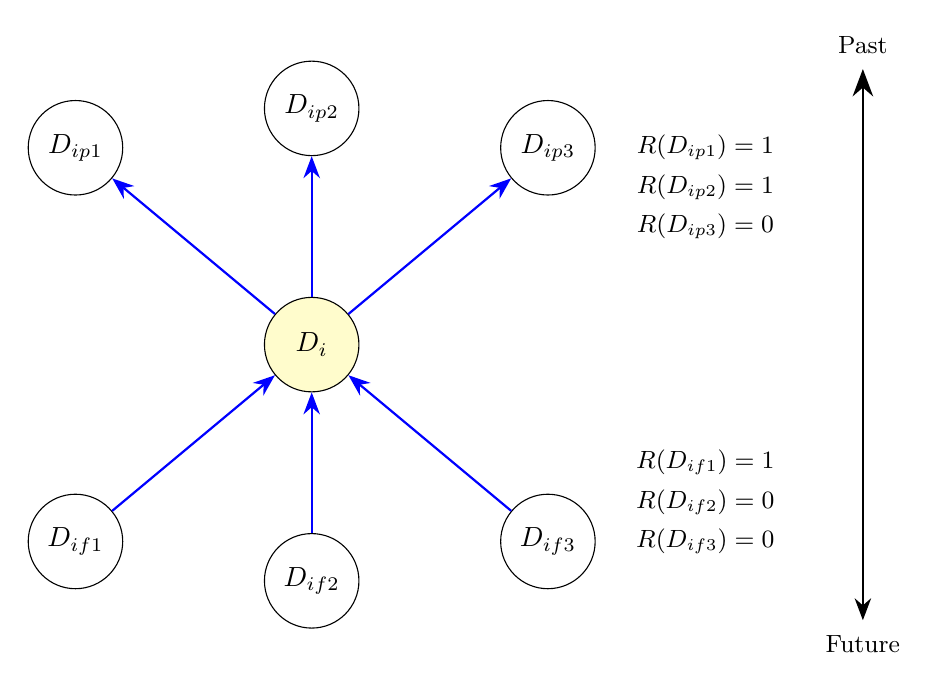
\begin{tikzpicture}[
    > = {Stealth[scale=1.2]},
    vertex/.style = {circle, draw, minimum size=1.2cm, inner sep=1pt},
    ref_edge/.style = {->, thick, blue},
    label_style/.style = {font=\small}
]

% Main document Di
\node[vertex, fill=yellow!20] (Di) at (0,0) {$D_i$};

% Past references (Dip) - More fanned out
\node[vertex] (Dip1) at (-3,2.5) {$D_{ip1}$};
\node[vertex] (Dip2) at (0,3) {$D_{ip2}$};
\node[vertex] (Dip3) at (3,2.5) {$D_{ip3}$};

% Future references (Dif) - More fanned out
\node[vertex] (Dif1) at (-3,-2.5) {$D_{if1}$};
\node[vertex] (Dif2) at (0,-3) {$D_{if2}$};
\node[vertex] (Dif3) at (3,-2.5) {$D_{if3}$};

% Edges for past references
\draw[ref_edge] (Di) -- (Dip1);
\draw[ref_edge] (Di) -- (Dip2);
\draw[ref_edge] (Di) -- (Dip3);

% Edges for future references
\draw[ref_edge] (Dif1) -- (Di);
\draw[ref_edge] (Dif2) -- (Di);
\draw[ref_edge] (Dif3) -- (Di);

% Labels for sets
% \node[label_style] at (-4,2) {$D_{ip}$ (Referenced by $D_i$)};
% \node[label_style] at (-4,-2) {$D_{if}$ (References to $D_i$)};

% Relevancy function examples
\node[label_style] at (5,2.5) {$R(D_{ip1}) = 1$};
\node[label_style] at (5,2) {$R(D_{ip2}) = 1$};
\node[label_style] at (5,1.5) {$R(D_{ip3}) = 0$};
\node[label_style] at (5,-1.5) {$R(D_{if1}) = 1$};
\node[label_style] at (5,-2) {$R(D_{if2}) = 0$};
\node[label_style] at (5,-2.5) {$R(D_{if3}) = 0$};

% Time arrow (vertical)
\draw[{Stealth[scale=1.5]}->, thick] (7,3.5) -- (7,-3.5);
\node[label_style] at (7,3.8) {Past};
\node[label_style] at (7,-3.8) {Future};

\end{tikzpicture}
\end{center}

These citation networks are rich in relevant documents, much more so than that of the document collection, which is demonstrated by the author comparing precision of pools using BCS and FCS against that of the entire document collection in Figure \ref{fig:citation-network-mining}. The logical, and simple augmentation of the encoder CAL approach would be to exhaust both BCS and FCS networks of a seed document prior to initiating the encoder CAL process. 

The theoretical benefits of citation network mining are that it can be used to augment the CAL process in ways that overcome some of the limitations of this process.  Firstly, CAL requires labelled data to train a classifier model, which is assumed to perform better with more data points. Encoder CAL approaches suffer disproportionately to that of feature-based CAL approaches due to their need for larger amounts of training data to effectively learn meaningful representations. This is because encoder models like BERT need to learn complex contextual relationships between words and concepts, whereas feature-based models can rely on simpler statistical patterns. When working with limited labeled data in the early stages of screening, encoder models may struggle to generalise well, potentially leading to suboptimal performance in identifying relevant documents. As discussed in the Encoder CAL process, often a single sample seed document is used during the first epoch for fine-tuning. A better approach would be to exhaust the citation network of that seed document first for labelling, before using revealed relevant documents to fine-tune the model, potentially resulting in a more performant model at the earlier stages of screening with less oracle cost. 

\subsubsection{Extending current citation network mining approaches}

BCS and FCS citation network mining faces a significant limitation in its inability to identify indirect citation relationships. An indirect citation occurs when research papers are connected through intermediate references, forming a chain of citations rather than a direct reference. For instance, when document $D_i$ cites document $D_{ip1}$, which in turn cites document $D_{ip2}$, a relationship exists between $D_i$ and $D_{ip2}$ despite the absence of a direct citation. This relationship represents an indirect citation, which is shown in Figure \ref{fig:indirect-citation}. This causes issues if $D_{ip1}$ is not included in the document pool, as $D_i$ and $D_{ip2}$ will no longer have an edge. 

This constraint makes it unsuitable as a complete solution for document relationship discovery for the encoder CAL process. However, researchers have proposed several modifications to the citation network mining process to address this limitation:

\begin{center}
    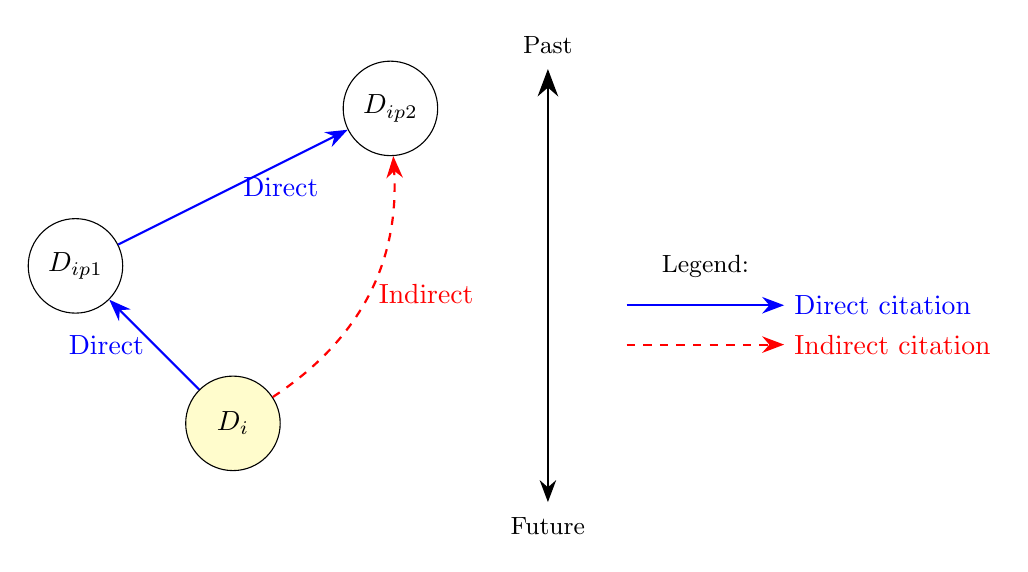
\begin{tikzpicture}[
        > = {Stealth[scale=1.2]},
        vertex/.style = {circle, draw, minimum size=1.2cm, inner sep=1pt},
        ref_edge/.style = {->, thick, blue},
        indirect_edge/.style = {->, thick, red, dashed},
        label_style/.style = {font=\small}
    ]
    
    % Main document Di
    \node[vertex, fill=yellow!20] (Di) at (0,0) {$D_i$};
    
    % Direct reference
    \node[vertex] (Dip1) at (-2,2) {$D_{ip1}$};
    
    % Indirect reference
    \node[vertex] (Dip2) at (2,4) {$D_{ip2}$};
    
    % Add edges
    \draw[ref_edge] (Di) -- (Dip1) node[midway, left] {Direct};
    \draw[ref_edge] (Dip1) -- (Dip2) node[midway, right] {Direct};
    \draw[indirect_edge] (Di) to[bend right] node[midway, right] {Indirect} (Dip2);
    
    % Time arrow (vertical)
    \draw[{Stealth[scale=1.5]}->, thick] (4,4.5) -- (4,-1);
    \node[label_style] at (4,4.8) {Past};
    \node[label_style] at (4,-1.3) {Future};
    
    % Legend
    \node[label_style] at (6,2) {Legend:};
    \draw[ref_edge] (5,1.5) -- (7,1.5) node[right] {Direct citation};
    \draw[indirect_edge] (5,1) -- (7,1) node[right] {Indirect citation};

    \end{tikzpicture}

    \label{fig:indirect-citation}
    \end{center}


\begin{itemize}
    \item \textbf{Matching isolated nodes based on similarity metric of their embeddings}: If $N$ is all the documents in the total pool, and $N_{isolated}$ is the set of documents that are not cited by any other document in $N$, then for each document $D_{ip} \in N_{isolated}$, find the document $D_i \in N$ with the highest similarity metric (i.e. cosine similarity) to $D_{ip}$. Add a artificial edge between $D_i$ and $D_{ip}$.
    \item \textbf{Matching isolated compoments on similarity metric of their embeddings}: When analyzing document clusters, some small groups of documents (called isolated components) may be disconnected from the main cluster. These isolated components have fewer connections to other documents, which can reduce classification accuracy. To fix this:
    \begin{itemize}
        \item Identify isolated components $C_{isolated}$ that have fewer or equal nodes than the main cluster
        \item For each node in these isolated components
        \item Calculate a similarity metric (i.e. cosine similarity) to nodes in larger clusters $C_i$
        \item Connect it to the most similar large cluster by adding a artificial edge
    \end{itemize}

\end{itemize}

This constraint however doesn't make it unsuitable as a partial improvement to the encoder CAL process for identifying relevant documents based on the initial seed document. Even without considering indirect citations, assessing the citation network of the seed document is potentially more relevant than that of the entire document collection. In table \ref{tab:citation-network-mining} it is unequivacle that the precision of relevant documents within pools using BCS, FCS  and both together against that of the entire document collection is much higher.

\hl{Make this data!}

\begin{table}[h]
    \centering
    \caption{Precision of relevant documents within pools using BCS, FCS and both together against that of the entire document collection}
    \label{tab:citation-network-mining}
\end{table}

\subsubsection{Research Question 1}

As outlined above, current approaches to encoder-based medical CAL rarely or indirectly leverage BCS/FCS as an initial expansion to relevant documents. Yet, BCS and FCS are known to yield high-precision citation pools, which could jumpstart the learning process. Therefore, the first research question is: {\it{To what extent can leveraging BCS and FCS before initiating an encoder-based CAL pipeline improve precision in identifying relevant medical research articles?}}

The proposed methodology would be to use the CLEF dataset, for which document relations could be extracted from forming a citation network using the opensource OpenAlex API\footnote{https://openalex.org/docs/api}. A variety of seeds of known relevant documents would be used to form the initial BCS/FCS citation pools, which would be used initially within the encoder-based CAL process. The aim would be to have citation pools that have varying sizes (denoted by the number of nodes within the citation pool), so that the performance of different citation pool sizes can be compared. This could be achieved by creating a citation pool for every known relevant document using the OpenAlex API, which can be parralised across multiple threads. From the list of citation pool sizes, seeds would be selected from the lower, middle and upper ranges of the list. 

After exhausting the citation network of the seed documents, the process would continue with the standard encoder-based CAL process, up to a maximum number of iterations. 



Datasets: CLEF
Seeds: A selection of seeds denoting known relevant documents.

Backward and forward citation pool construction


Experimental design

Citation Augmented considerations
Baseline considerations
Evaluation metrics
Ablation studies
BCS - only vs FCS only vs BCS+FCS expansions
Varying seed sizes (1 vs 5 vs 10 known relevant documents)
Analysis plan: 
Check to see how quickly each approach achieves a given level of prevision
Computational costs - measure how much computational resources are required to achieve a given level of precision
Citation network density - Correlate the final performance with the desnsity / size of the BCS/fcs network to understand if a bigger BCS/FCS network leads to better performance.

    
\subsubsection{Graph Neural Networks}

    A research paper is a rich source of information, and contains multiple features that can be used to represent that document, however in the title and abstract screening phase, it is limited to only using the title and abstract features. As the previous research area aims to demonstrate, utilising other features could improve the precision of the encoder CAL process, so, logically utilising more features could improve the precision of the encoder CAL process further. 

    Previous work by this author has demonstated that features about authors, primary topic and publication date all impact classification accuracy. \hl{link this to the retraction watch paper}

    In-keeping with the above research theme, graph neural networks offer a natural extension to considering additional document features, and still being able to utilise the structural information about relationships between documents. 

    
    \subsubsection{LLMs and citation network mining}

    The motivation for using LLMs and graph networks is to combine the structurality of graph citation networks with the ability of the LLMs to comprehend the semantic meaning of documents. As outlined, citation network graph analysis occurs above the document level through utilisation of extracted features about documents. LLMs are a natural replacement for extraction of features, as they possess the ability to understand semantic meaning of documents. The ultimate goal to use LLMs and graph networks is to complment and enhance isuses with the other. 

    Research has been conducted into the use of LLMs within the graph neural networks, and has developed a robust taxonomy for categorising the use of LLMs within graph networks \cite{llm4g}. 
    
    The first application of LLms within graph networks is to use LLM as an enchancer. Typically graph neural networks encode text into nodes using simple bag-of-words, skip-gram or TF-IDF. LLMs are able to encode text into nodes using more complex features, such as semantic meaning, which can be used within the graph neural networks. This can be further subdivided into explanation based and embedding based enchancers. 
    
    Explanation based enhancers query an LLM using prompting to capture higher level features about documents, which is used to enrich node representations prior to processing with a graph neural network, with the process being abstracted in in Figure \ref{fig:llm4g}. The approach used by https://arxiv.org/pdf/2305.19523 was to prompt GPT 3-5 with the abstract and text of a document along with a questions about that document using a zero-shot approach. The LLM reponse then forms features which are amended to the original node representations. Issues with this approach is that this requires domain specific knowledge, as features which are deemed important (and hence prompt used) are dependent on the domain of the research. It was performant on the pubmed domain, scoring greater node classification accuracy using this approach (0.9618 $\pm$ 0.0053) than utilising an LLM alone on pubmed data (0.9494 $\pm$ 0.0046).   

    \begin{figure}[h]
        \centering
        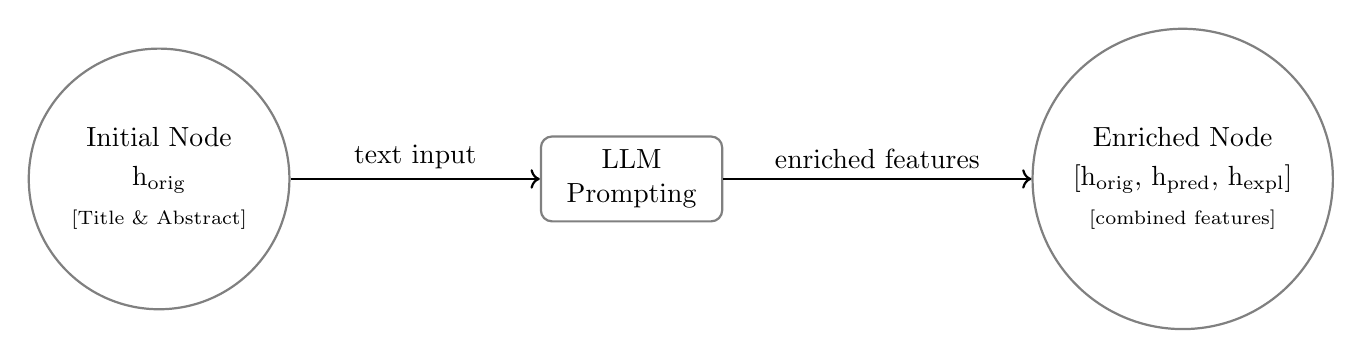
\begin{tikzpicture}[node distance=3cm,auto]
        
        % Define styles
        \tikzstyle{node} = [circle, minimum width=2.5cm, minimum height=2.5cm, draw=black!50, thick]
        \tikzstyle{process} = [rectangle, rounded corners, minimum width=2cm, minimum height=1cm, draw=black!50, thick]
        \tikzstyle{features} = [text width=2cm, align=left]
        
        % Initial node
        \node[node] (initial) {
            \begin{tabular}{c}
                Initial Node\\[2pt]
                h\textsubscript{orig}\\[2pt]
                \scriptsize{[Title \& Abstract]}
            \end{tabular}
        };
        
        % Process box
        \node[process, right of=initial, xshift=3cm] (process) {
            \begin{tabular}{c}
                LLM \\Prompting
            \end{tabular}
        };https://arxiv.org/pdf/2305.19523 was to prompt GPT 3-5 with
        the abstract and text of a document along with a questions about that document using a zero-shot approach. The
        LLM reponse then forms features which are amended to the original node representations. Issues with this approach
        
        % Enriched node
        \node[node, right of=process, xshift=4cm] (enriched) {
            \begin{tabular}{c}
                Enriched Node\\[2pt]
                [h\textsubscript{orig}, h\textsubscript{pred}, h\textsubscript{expl}]\\[2pt]
                \scriptsize{[combined features]}
            \end{tabular}
        };
        
        % Arrows
        \draw[->, thick] (initial) -- (process) node[midway, above] {text input};
        \draw[->, thick] (process) -- (enriched) node[midway, above] {enriched features};
        

        
        \end{tikzpicture}
        \caption{Node feature enrichment process using LLM and LM}
        \label{fig:llm4g}
        \end{figure}

    \subsubsection{Research Question 2}

    Proposal: Utilising more features in the encoder CAL process can improve the precision of the encoder CAL process.

    \newpage

    \subsection{Utility Based Stopping Algorithms}


\section{DATASETS}


Numerous data sets related to this area have been used in the existing literature.

\subsection{CLEF-TAR (2017, 2018, 2019)}

CLEF-TAR is a dataset that was released as part of CLEF eTASK 2, and is available on github\footnote{https://github.com/CLEF-TAR/tar} \cite{kanoulas_clef_2017, kanoulas_clef_2018, kanoulas_clef_2019}. Originally designed with document ranking as the primary focus, the information contained within the data set allows for the subprocess simulation of the title and abstract selection of the SR procedure, using published real-world Cochrane SRs. Each year, this data set was incrementally updated and Table \ref{tab:training_dataset_clef} outlines the scope of the issue and succinctly highlights the presence of a large imbalance of the TIR class. Diagnostic test accuracy SRs (DTA) summarise a test accuracy, while intervention reviews assess the effectiveness/safety of a treatment, vaccine, device, preventative measure, procedure, or policy. Delineation between the types of SRs is not required for research within this Ph.d.


\begin{table*}
    \centering
    \begin{tabular}{|c|c|c|c|c|c|}
    \hline
        Dataset & Total SRs & Type(s) of SR & T & TR & TR/T\\   \hline
        CLEF 2017 & 50 & DTA & 269628 & 4661  & 0.017 \\   \hline
        CLEF 2018 & 50 & DTA & 266657 & 4351 & 0.016\\   \hline
             CLEF   2019 & 80 & DTA & 485153 & 8315 & 0.017\\   \hline
               CLEF  2019 & 80 & Intervention & 31644 &  448 & 0.014 \\   \hline
Synergy & 26 & Not Applicable & 169288 &  2834 & 0.017 \\   \hline
    \end{tabular}
    \caption{Training Dataset sizes for the TAR datasets}
    \label{tab:training_dataset_clef}
\end{table*}

Of importance, the CLEF dataset did not provide the titles or abstracts for each research found in the Identification Phase, rather relying on the users to download them for experimentation. This is an important oversight of the data set as titles and abstracts can be updated or retracted post-publication, meaning, fair comparison across time might become increasingly challenging. Within this Ph.D. I intend to use this recently collected source \(2024\) of titles/abstracts that have been collected as part of other work in this area, which has extracted all titles and abstracts for \(\textbf{T}\) within the CLEF dataset \cite{goharian_reproducibility_2024}\footnote{https://github.com/ielab/goldilocks-reproduce}.

\subsection{Synergy Dataset}
The Synergy dataset \cite{de_bruin_synergy_2023}, while less frequently used in the literature, offers a more contemporary collection of SRs\footnote{https://github.com/asreview/synergy-dataset/tree/master}. This data set comprises 26 SRs that span multiple domains, with a predominant focus on the medical field (20 out of 26 reviews). Reviews included in this data set range from 2002 to 2020, potentially providing more recent information compared to the CLEF data set.
The Synergy data set features diverse domains, allowing cross-domain analysis despite its primary focus on medical reviews. It also includes an expanded variable set. In addition to the basic information found in the CLEF dataset, Synergy incorporates authorship details, referenced works, and publication years, all sourced from the OpenAlex API.
Due to its more recent compilation and limited use in existing research, this dataset could be used to externally validate pre-trained language models.The inclusion of SRs from nonmedical domains, such as computer science, allows evaluations on the transferability of TAR approaches across different fields.
Synergy's TR/T ratio of 0.017 is consistent with the class imbalance observed in the CLEF datasets, making it suitable for comparative studies and model evaluation in the context of title and abstract selection tasks.

\subsection{TREC Total Recall Track Dataset (2015, 2016)}
The TREC Total Recall Track produced data sets specifically designed for high-recall retrieval tasks, similar to those encountered in SRs\footnote{https://trec.nist.gov/data/total-recall/}\cite{roegiest_trec_2015, grossman_trec_2016}. This data set simulates scenarios where the goal is to find all or nearly all relevant documents in a collection, which aligns closely with the objectives of the title and abstract screening phase in SRs. The data set includes a corpus of documents, topics (which can be seen as analogous to research questions in SRs), and relevance judgments.

\subsection{Jeb Bush Emails Dataset}
The Jeb Bush Emails dataset is an unconventional choice for TAR research, originally consisting of emails released by former Florida Governor Jeb Bush\footnote{https://ab21www.s3.amazonaws.com/JebBushEmails-Text.7z}. This data set is suitable for TAR experiments because of its large size and the presence of both relevant and irrelevant documents. Although not directly related to SRs, it provides a real-world corpus that can be used to simulate document classification tasks inherent in the SR process.

\subsection{RCV1-v2 Dataset}
The RCV1-v2 (Reuters Corpus Volume 1, Version 2) is a large, manually categorised newswire data set \cite{lewis_rcv1_2004} that was published by Reuters between August 20, 1996, and August 19, 1997\footnote{https://github.com/scikit-learn/scikit-learn/blob/main/sklearn/datasets/\_rcv1.py}. The dataset features 804,414 documents with multi-label classification across 103 topic categories, organised in a hierarchy. The documents are provided in XML format with rich metadata and the content is primarily English news stories covering a wide range of topics.
Although not originally designed for SRs, RCV1-v2 has been used in various text classification and information retrieval tasks.  In the context of SRs and TAR, the use of the RCV1-v2 data set lies in the simulation of approaches on a large-scale dataset to test the scalability and efficiency of screening algorithms and to evaluate any potential transferability of the approaches.

RCV1-v2 dataset is adapted for use in AL by denoting all documents as \textbf{$T$}, \textbf{$T_R$} as all documents having a specific label, and those without it, as by treating the entire corpus as \textbf{$T$}, \textbf{$T_{IR}$}, we can approximate the binary classification challenge of title and abstract Screening within SRs.

\section{Evaluation Metrics}
Evaluation metrics for SR TAR process can be categorised between assessing how well a classifier minimised the relevant documents excluded by the classifier with a set work budget (i.e. effectiveness) or the reduction in the reviewer's workload by excluding the maximum number of irrelevant documents while maintaining recall (efficiency).  The majority of the research produced within this will focus on improving the effectiveness of AL models within the medical TAR domain. The author chooses not to optimise the computational efficiency between approaches, rather to improve the final result achieved. This is for numerous reasons; however, the main two are that as computer processing increases, these practical limitation concerns become less and improvement in effectiveness will have a greater impact on SR usefulness than maximising efficiency.  The author aims to report the time taken to run the algorithms, time complexity and the hardware that ran upon, so that comparison to time taken by humans undertaken can occur.

\subsection{Recall@k}
In the context of SRs, achieving high recall is more critical than high precision. Recall represents the proportion of relevant documents correctly identified among all truly relevant documents \cite{omara-eves_using_2015}. This focus on recall may seem counterintuitive, but it is crucial for two reasons. First, each missed document could potentially contain significant information for the SR. Second, the initial screening is followed by a more precise full-text review (as outlined in the PRISMA workflow, Figure \ref{fig:selection_and_screening}), where precision is emphasised.
Although maximising recall is important, it is not practical to aim for 100\% due to diminishing returns. As recall approaches higher levels, the computational cost of screening additional documents increases substantially, often yielding minimal benefit. To balance effectiveness and efficiency, researchers of TAR for SR commonly use and consider recall @ 95\% as useful (that is, k = 0.95). This measure indicates the recovery achieved when 95\% relevant documents are recovered, striking a pragmatic balance between comprehensive coverage and resource use. A higher recall@k is considered a more effective approach.
Recall is calculated via:

\begin{equation}
\text{recall} = \frac{\text{TP}}{\text{TP} + \text{FN}}
\end{equation}
Recall@95\% is calculated via:
\begin{equation}
\text{recall@95\%} = \frac{\text{TP}}{\text{TP} + \text{FN}}
\end{equation}
Where recall is calculated once an AL classifier achieves 95\% TP.

A small point on nomenclature: Historically, recall has been referred to in the medical literature as sensitivity. These are two different terms for the same metric, and the use of either term depends on the domain. Additionally, in the legal domain, there might be references to recall@75\% which is not as useful for the medical domain. Legal domains often prioritise based on cost-effectiveness, time-constraints and proportionability, which medical reviews require as close to absolute information as possible \cite{tsafnat_systematic_2014}.

\subsection{R-Precision}
This effectiveness metric determines, given the \textbf{$T_R$}, what proportion of documents returned by the approach within the total number of relevant documents were actually relevant \cite{manning_introduction_2008}. The best score for R-precision is 1 (i.e., all relevant documents were returned in the top \textbf{$T_R$} position). It allows for an adaptive cutoff for \textbf{$T_R$}, which adapts to the SR, and also considers precision. Note that this evaluation metric can only be used when the \textbf{$T_R$} for a query is known. It is calculated via:

\begin{equation}
\text{R-Precision} = \frac{\text{Relevant Documents in top } T_R}{T_R}
\end{equation}
\subsection{Work Saved Over Sampling (WSS@k)}

WSS@k is an efficiency metric that would be valuable to report on to enable other researchers in the field to compare their approaches to mine and, if appropriate, improve upon. Again, k (recall) is typically set to 0.95. This metric evaluates the work saved over random sampling, with a higher WSS@k being more efficient and is calculated via:


\begin{equation}
\text{WSS} = \frac{\text{TN} + \text{FN}}{\text{T} - (1 - \text{Recall})}
\end{equation}
% \begin{equation*}
% \lightshadowbox{\text{WSS} = \frac{\text{(TN + FN)}}{\text{T - (1 - Recall)}}
% \end{equation*}

This can also be expressed as:
\begin{equation}
\text{WSS} = \frac{\text{TN} + \text{FN}}{\text{T} - 1 + \frac{\text{TP}}{\text{TP} + \text{FN}}}
\end{equation}
% \begin{equation*}
% \lightshadowbox{\text{WSS} = \frac{\text{TN + FN}}{\text{T} - 1 + TP/(\text{TP + FN})}
% \end{equation*}

%%%%%%%%%%%%%%
% References
%%%%%%%%%%%%%%

\printbibliography
\end{document}

